% LaTeX source generated from paperE1_cod_forecast_ladder_v15.md by wave13/build_latex_v13.py (batch 7 (audits of agent arena 1 paper rewrites)/wave13).
% Pandoc body identical to the wave-9/11 output (asserted at build time), with the
% declaration subsections relocated to a trailing Declarations section.
% Front matter: Amin Abaee, Independent Researcher, clickable ORCID
%(https://orcid.org/0000-0002-0019-1842) and email (amin_abaee@ut.ac.ir)
% beneath the name; date September 6, 2026.
% Back matter: the paper's own declarations, each a titled subsection, plus
% the AI declaration (GLM (Z.ai), Qwen (Alibaba Cloud) and DeepSeek AI
% assisted with drafting and iterative review).
% References carry the owner's Zenodo DOIs (see wave13/apply_md_doi.py).
% Edit the markdown source and re-run the build script to regenerate.
% Compiles error-free with tectonic (also compatible with pdflatex/xelatex).
\documentclass[11pt]{article}
\usepackage[a4paper,margin=1in]{geometry}
\usepackage{amsmath,amssymb}
\usepackage{graphicx}
\usepackage{booktabs,longtable,array,calc}
\usepackage{xcolor}
\usepackage[colorlinks=true,allcolors=blue!45!black]{hyperref}
\usepackage[font=small,labelfont=bf]{caption}
\usepackage{etoolbox}
\AtBeginEnvironment{longtable}{\small}  % dense data tables
\setlength{\tabcolsep}{4pt}
\providecommand{\tightlist}{\setlength{\itemsep}{0pt}\setlength{\parskip}{0pt}}
\setcounter{secnumdepth}{-1}
\emergencystretch=3em
\graphicspath{{../}}
\begin{document}
\title{Does a surplus-production ladder improve forecasts of Northern cod? A scored test on NAFO 2J3KL}
\author{Amin Abaee\\[0.35em]
{\small Independent Researcher}\\[0.55em]
{\small\href{https://orcid.org/0000-0002-0019-1842}{ORCID: 0000-0002-0019-1842}}\\[0.3em]
{\small\href{mailto:amin\_abaee@ut.ac.ir}{amin\_abaee@ut.ac.ir}}}
\date{September 6, 2026}
\maketitle

{\centering\small \textbf{Prepared in the format of Fisheries Research}\par}

\subsection{Highlights}\label{highlights}

\begin{itemize}
\tightlist
\item
  A five-module structural ladder is scored against two naive baselines
\item
  No module attains lower pooled rolling-origin RMSE than persistence
\item
  From a pre-collapse origin, every model misses the 1991--1995 collapse
\item
  No module is retained, scoped to the estimator and series tested
\item
  Stall reconstructions and the ladder share the constant-productivity
  failure mode
\end{itemize}

\begin{abstract}

Five surplus-production modules and two naive baselines are scored on
Northern cod (\emph{Gadus morhua}), NAFO 2J3KL, under a rule whose
scoring core was fixed beforehand: a module is kept only if it lowers
RMSE against the next-simpler module and persistence. The predictand is
NCAM M-shift SSB (DFO, 2016, Table A2), 1983--2015, LRP 884.6 kt.

No module is retained on these two unpooled series, on rolling RMSE
pooled over origins within each specification and horizon: under the
primary coarse pass one-year RMSE is 98 kt for persistence against
115--196 kt, five-year 265 against 289--488 kt. By period the ordering is not uniform. From the fixed pre-collapse origin every model misses the 1991--1995
collapse (694--819 kt against 670 and 688 kt for baselines): constant
productivity with a 1992 catch drop cannot reproduce it. Added structure
is not uniformly harmful, yet none closes the gap. A second, unpooled specification (xteNCAM, 1954--2024, LRP 276 kt) gives
the same outcome (matched persistence 84 kt against M1's 120).

Simulation under known ground truth retains a true autonomous module in
97\% of replicates at collapse-window parameters but has power below
15\% for the stock-flow and depensation alternatives at recovery-window
parameters; the residual and lagged-initialisation modules were not
simulated. No Specification A margin against
persistence has an interval excluding zero, though several on
Specification B do. The predictand is retrospectively reconstructed rather than the vintages
at each origin, and catch is supplied along the horizon: a conditional
hindcast, not an operational forecast.

\end{abstract}

\textbf{Keywords:} northern cod; biomass forecasting; surplus
production; forecast evaluation; stock assessment; prediction skill;
model identifiability

\subsection{1. Introduction}\label{introduction}

Fisheries assessment builds structure by default. State-space
age-structured assessments, surplus-production models, and
ecosystem-linked extensions each add parameters, state variables, or
couplings in the hope of better advice. In the surplus-production implementations evaluated here, that structure
does not pay for itself: across a five-module ladder scored on two
unpooled assessment specifications, no tested implementation attains
lower pooled rolling-origin RMSE than last-value persistence at either
evaluated horizon. Split by period the pooled result is not uniform ---
persistence is not the lowest-error rule during the collapse band ---
and Section 3.5 reports that split. The result is scoped to the estimators and
series tested, and the exercise is a conditional hindcast rather than
an operational forecast test. Whether that structure improves
out-of-sample forecasts --- as opposed to in-sample fit --- is a
separate, testable question, and on it the burden of proof sits with the
added structure.

That burden is now formalised in assessment practice. Comparison against
a naive baseline has become a standard acceptance diagnostic: hindcast
cross-validation scores a model's out-of-sample predictions with the
mean absolute scaled error (MASE) of Hyndman and Koehler (2006), which
divides prediction error by the error of a random-walk forecast, so that
a value above one means the model predicts less accurately than assuming
no change (Kell et al., 2016; Kell et al., 2021). The diagnostic
cookbook of Carvalho et al. (2021) lists prediction skill so measured as
one of four criteria for accepting an integrated assessment, alongside
convergence, fit, and retrospective consistency, and the good-practice
guidance for surplus-production models adopts the same test (Kokkalis
et al., 2024). The reference forecast in that literature is therefore
already the one used here.

Two features of that practice leave the present question open. First,
MASE is almost always computed on the \emph{abundance index} a model
fits, not on the estimated stock state that advice is written about, so
a model can pass on the index it was tuned to while its biomass
trajectory remains untested. Second, the diagnostic is applied to
certify a single accepted assessment rather than to rank a graded
sequence of structural additions against each other and against the
naive rule at once. What is missing is a direct, scored comparison in
which the predictand is the assessment's own biomass output, each
increment of structure has a declared comparator, and the naive rule is
a competitor rather than a scaling constant. That is the comparison
reported here.

Northern cod (\emph{Gadus morhua}) in NAFO divisions 2J3KL is the
canonical demanding case. The late-1980s and early-1990s collapse --- a
spawning stock falling from a high, weakly trending phase to a few
percent of its 1980s mean --- occurred under an assessment and
management regime whose failures were dissected in the canonical
post-mortems (Hutchings and Myers, 1994; Walters and Maguire, 1996). The
non-recovery that followed the July 1992 moratorium has kept the
depensation question open for three decades (Shelton and Healey, 1999).
A partial rebuilding was documented in the 2010s (Rose and Rowe, 2015),
but surplus production has since stalled, with some years being negative
(Rose, 2026).

The measured quantity throughout is the condition of the productive
stock --- the spawning-stock biomass whose persistence underwrites
future yield. This is distinct from the catch taken from it. A fishery
can return a high extracted yield while the stock that produces it
declines, and it is the latter that the forecast here must track. Any
model family proposed for this stock must therefore first clear a
minimal bar: it must at least beat the forecast that nothing changes.
One-dimensional autonomous surplus-production maps carry a structural
constraint under sustained constant catch, discussed with its fitted
values and its scope in Section 4. It is a property of a map held at a
fixed removal level, not a reason the forecasts below fail, and the
scored comparison does not isolate it.

This evaluation follows a stated retention rule whose scoring core was
coded before the first scoring pass and applied unchanged (Section 4 records its protocol
status): additional model structure is retained only when it reduces
primary RMSE relative to the next-simpler model and relative to
persistence (\S{}2.3). Early-warning and intervention-selection criteria
are secondary objectives; neither is operationalised here (the
Brier score is reported as a secondary diagnostic and never changes a
retention verdict, and the moratorium is deliberately not evaluated).
The instrument is a forward-ordered ladder of surplus-production models
(not a strict nesting for M2 and M4) evaluated against two naive
baselines. It runs output-only, stock-and-flow, residual, then lagged initialisation;
prey- and index-informed observation variants are evaluated separately
in Section 3.4 and are not part of the ladder. A module is kept only if
it improves the stated score.

The paper asks whether stock-flow, residual, delay, or prey-informed
modules reduce SSB forecast error relative to last-value persistence and
to the autonomous surplus-production model. The scope is deliberately
narrow: this paper does not estimate an Allee threshold, identify the
cause of the 1990s collapse, or evaluate whether the 1992 moratorium was
adequate.

The stock was selected because of its data availability (a full
state-space assessment series), its policy relevance, and the sharpness
of its collapse-and-stall trajectory. The same scored design is applied to a groundwater system, the Edwards
Aquifer, Texas, in Abaee (2026a). The two systems' series are not
pooled, and no retention outcome is transferred between them.

The remainder of the article is organized as follows. Section 2 states
the data, the two assessment specifications, the model ladder, and the
evaluation design. Section 3 reports the results: the primary
specification (3.1), annual landings and the survey-start variant (3.2),
the alternative assessment specification (3.3), prey-informed
productivity (3.4), the Diebold--Mariano and block-bootstrap
uncertainty analysis (3.5), and the fitted parameters (3.6).
Section 4 discusses the findings, the identification limits, the
reconstruction-level corroboration, and the protocol status.
Section 5 concludes.

\subsection{2. Material and methods}\label{material-and-methods}

\subsubsection{2.1 Data and
specifications}\label{data-and-specifications}

The specification tables type each field as follows: D, data; E,
empirical construct; M, model; N, normative threshold.

\textbf{Table 1.} Primary specification --- Specification A (the
1983--2015 NCAM M-shift SSB series of DFO, 2016, Table A2; the
state-space assessment model of Cadigan, 2016).

\begin{longtable}[]{@{}
  >{\raggedright\arraybackslash}p{(\columnwidth - 4\tabcolsep) * \real{0.3333}}
  >{\raggedright\arraybackslash}p{(\columnwidth - 4\tabcolsep) * \real{0.3333}}
  >{\raggedright\arraybackslash}p{(\columnwidth - 4\tabcolsep) * \real{0.3333}}@{}}
\toprule\noalign{}
\begin{minipage}[b]{\linewidth}\raggedright
Field
\end{minipage} & \begin{minipage}[b]{\linewidth}\raggedright
Contents
\end{minipage} & \begin{minipage}[b]{\linewidth}\raggedright
Type
\end{minipage} \\
\midrule\noalign{}
\endhead
\bottomrule\noalign{}
\endlastfoot
System & Northern cod, NAFO 2J3KL, as represented by NCAM M-shift SSB &
D \\
Interest & Continuity of a spawning stock on the 2016
precautionary-approach cautious or healthy side of the 2016 LRP & N \\
Domain & Stock area in DFO (2016) Figure 1; calendar years 1983--2015 &
D \\
Safe set & \(S_t \ge \mathrm{LRP} = 884.6\) kt (1983--1989 mean of Table
A2) & N \\
Disturbance & Unspecified productivity shocks; not a fitted \(M(t)\) &
M \\
Theoretical catch & Any \(C_t \ge 0\) & M \\
Implementable catch & Pre-1992 directed fishery; post-2 July 1992
moratorium and low inshore removals & E \\
Horizon & Hindcast 1983--2015; two fixed test windows and rolling origin
& D \\
Food web & Capelin excluded from the primary pass; tested as a variant
in Section 3.4 & M \\
Norm & 2010/2016 DFO precautionary-approach LRP (1980s mean SSB), not
the 2023 40\% \(B_{\mathrm{MSY}}\) LRP & N \\
\end{longtable}

Table 1 note: the safe-set and LRP fields type the reference frame of
the evaluation; the primary RMSE score never uses them (only the
secondary Brier indicator score does).

Table A2 also reports fishing mortality \(F\) and natural mortality
\(M\). They are joint outputs with SSB and are not used as exogenous
inputs.

Regular et al.~(2025) extend the assessment to 1954, revise the LRP to
276 kt (95\% interval 180--423 kt; 40\% of \(B_{\mathrm{MSY}}\)), and
estimate 2024 SSB at 342 kt. That is a second specification ---
Specification B (the 1954--2024 extended xteNCAM series; Section 3.3).
The two objects differ in five specification fields: (1) the state
equation (xteNCAM versus NCAM M-shift), (2) the start year (1954 versus
1983), (3) the reference threshold (276 kt versus 884.6 kt), (4) the
treatment of catch, and (5) the horizon.
The two SSB columns are not mixed. The reconstructions are scored separately because they differ in
estimated SSB trajectory, assessment formulation, temporal coverage and
catch specification; the reference threshold enters only the secondary
classification diagnostic and not the primary RMSE comparison. No
retention outcome is carried from one specification to the other.

\subsubsection{2.2 Forecast models}\label{forecast-models}

Northern cod surplus production is represented as a discrete-time map,
with \(S\) in kt and \(C\) in kt yr\textsuperscript{-1}.

\textbf{Definition 2.1 (Surplus-production map).} The autonomous
surplus-production map with multiplicative depensation is

\[
\begin{gathered}
S_{t+1}=\bigl[S_t+g(S_t)-C_t+\varepsilon_t\bigr]_+,
\qquad
g(S_t)=rS_t\bigl(1-S_t/K\bigr)\,a(S_t),
\\
a(S_t)=
\begin{cases}
1 & \text{(Schaefer; no Allee term declared)},\\[2pt]
\dfrac{S_t-\mathfrak s}{K-\mathfrak s} & \text{(depensation term active, $\mathfrak s>0$)}.
\end{cases}
\end{gathered}
\]

Two conventions fix how this map is used. The disturbance
\(\varepsilon_t\) is a regression error at estimation only: parameters
are fitted to the one-step increments with \(\varepsilon_t\) as the
residual, and all forecasts reported here set \(\varepsilon_t = 0\), so
every forecast trajectory is a deterministic plug-in path rather than a
multi-step conditional mean, except in M3 and M4, which carry the
fitted residual forward as a state. In those two modules the training residuals are
\(e_u = \Delta S_u - [g(S_u) - C_u]\) over the training transitions,
formed before any clipping. The coefficient \(\hat\phi\) is the
no-intercept lag-one least-squares estimate
\(\sum_u e_u e_{u-1}/\sum_u e_{u-1}^2\); it is set to zero when the
denominator is not positive or the window supplies fewer than four
residuals, and is clipped to \([-0.95, 0.95]\). The residual carried
into the forecast is the last training residual \(e_{\mathrm{last}}\),
and the projected residual at step \(k \ge 1\) is
\(\hat\phi^{\,k} e_{\mathrm{last}}\), added inside the update before
the state is clipped to \([10^{-3}, 10^{6}]\) kt.
Catch is dated so that \(C_t\) is the catch taken during the interval
from \(t\) to \(t+1\); a forecast issued at origin \(t\) therefore
uses the recorded catch for the year it is forecasting. Under the
coarse regime this places the 1992 drop in the step from 1992 to 1993,
so on the fixed collapse test window (1991--1995) the drop does not
enter the first two forecast steps; the models are already rising before
it applies.
For multi-step forecasts the catch path is supplied for the
whole horizon, so the exercise is a conditional hindcast with respect to
catch, not an operational forecast; Section 4 returns to this.

The factor \(a(S_t)\) is a multiplicative depensation term, not a
parameter switch. Setting \(\mathfrak s=0\) gives \(a(S_t)=S_t/K\) (a
cubic modification of the logistic surplus), not the Schaefer law. The
Schaefer model is the separate member of the family in which the factor
is replaced by \(1\); Abaee (2026b) makes the same distinction.

Section SI-2 gives the statement and proof.

The model ladder is given in Table 2.

The ladder is the forward-ordered set of seven entries \(\{\)persist,
mean, M1, M1b, M2, M3, M4\(\}\) of Table 2, ordered by structural
complexity (autonomous surplus map, Allee extension, stock-flow,
residual, delay): two naive baselines (persist, mean) and five
structural modules. Where this article refers to a five-module ladder
evaluated against two naive baselines, it means this set. It is not a
strict nesting for M2 and M4.

\textbf{Table 2.} Model ladder.

\begin{longtable}[]{@{}
  >{\raggedright\arraybackslash}p{(\columnwidth - 6\tabcolsep) * \real{0.2500}}
  >{\raggedright\arraybackslash}p{(\columnwidth - 6\tabcolsep) * \real{0.2500}}
  >{\raggedright\arraybackslash}p{(\columnwidth - 6\tabcolsep) * \real{0.2500}}
  >{\raggedright\arraybackslash}p{(\columnwidth - 6\tabcolsep) * \real{0.2500}}@{}}
\toprule\noalign{}
\begin{minipage}[b]{\linewidth}\raggedright
ID
\end{minipage} & \begin{minipage}[b]{\linewidth}\raggedright
Class
\end{minipage} & \begin{minipage}[b]{\linewidth}\raggedright
Free on the training window
\end{minipage} & \begin{minipage}[b]{\linewidth}\raggedright
Frozen into the test window
\end{minipage} \\
\midrule\noalign{}
\endhead
\bottomrule\noalign{}
\endlastfoot
persist & baseline & --- & \(\hat S_{t+h}=S_t\) \\
mean & baseline & training mean &
\(\hat S_{t+h}=\bar S_{\mathrm{train}}\) \\
M1 & autonomous & \(r,K\); \(C\) = training-mean catch (plugged, not
estimated) & same \(C\) \\
M1b & autonomous with Allee & \(r,K,\mathfrak s\); \(C\) =
training-mean catch (plugged, not estimated) & same \(C\) \\
M2 & stock-flow & \(r,K\); \(C_t\) prescribed & prescribed \(C_t\) \\
M3 & residual & M2 + AR(1) residual & \(\phi\) persisted \\
M4 & lagged initialisation & \(r,K\) and \(\phi\) refitted exactly as for M3 & forecast
starts from \(S_{t-1}\) \\
\end{longtable}

The coarse catch regime, taken from DFO (2016) prose (the
precautionary-approach framework of DFO, 2009), is \(C_t=240\) kt for
\(t\le 1991\), \(C_t=120\) kt for \(t=1992\), and \(C_t=5\) kt for
\(t\ge 1993\). Year-by-year landings (Schijns et al., 2021, Table 1)
replace that regime in Section 3.2. Regular et al.~(2025) Table 1
matches Schijns exactly on 1983--1993 (11 years, maximum absolute
difference 0 t); STATLANT matches Schijns on 1983--1993, so the
STATLANT-versus-Schijns sensitivity is closed on 1983--1993 (they are
the same column there). The Specification A collapse test window runs to
1995, two years beyond the verified match; the residual exposure is
immaterial, since Schijns records 1.31 kt in 1994 and 0.41 kt in 1995
against a collapse-window \(\Delta S\) of hundreds of kilotonnes. A
1956 discrepancy between those sources (236,210 t versus 263,210 t) lies
outside the 1983--2015 Specification A range; Specification B begins in
1954 and so contains 1956, but it draws its catch column from the
xteNCAM reconstruction rather than from either of these two sources, so
the discrepancy is unused on both specifications. The coarseness of the regime series is a limitation.

Parameters are estimated by one-step least squares on the training
window only. Rolling-origin training windows expand rather than slide:
each origin refits on all history up to that origin, subject to the
minimum length. A window of \(m\) annual states supplies
\(m-1\) one-step transitions, and it is the transition count that sets
the effective regression sample. Bounds: \(r\in(0.001,2]\), and \(K\) constrained above the largest state
the one-step regression conditions on. The estimation code optimises
\(K\) on \([\max_{\mathrm{train}} S + 10, 5000]\) kt, where
\(\max_{\mathrm{train}} S\) is taken over the predictor states \(S_t\)
of the training transitions and so excludes the terminal state of the
window. Here \(500\) kt is the multi-start initialiser rather than the
lower bound, consistent with the frozen specification's constraint of
\(K\) above the training maximum.
The remaining estimation bounds are
\(\mathfrak s \in [0, \max_{\mathrm{train}} S_t]\) with the further
feasibility restriction \(0 < \mathfrak s < 0.8K\) enforced in the
objective, \(\phi\) clipped to \([-0.95, 0.95]\), and the index
exponent \(b\) fitted jointly with \(r\) and \(K\) without bounds.
The profile of Section 3.2 restricts \(\mathfrak s\) further, to
\([0, \min_{\mathrm{train}} S_t]\), for the reason given there. The
reported fits attain the upper endpoint (\(K = 5000\) kt) where the
objective is flat out to the imposed bound; M1b's recovery-window
\(K = 105.8\) kt is a valid interior fit, not a bound violation. Where a
reported fit sits at \(500.0\) kt this is the multi-start initialiser,
which the optimiser has not left because the objective is flat there,
and not an active constraint. M3's autoregressive coefficient is
estimated in a second stage: \(r\) and \(K\) are fitted first by
one-step least squares, and \(\phi\) is then obtained as the
lag-one regression coefficient of the resulting training residuals on
their own lag, clipped to \([-0.95, 0.95]\); it is not jointly
optimised with \(r\) and \(K\). Every
fitted-parameter value this article prints, with the window it belongs
to and the bound it attains, is collected in Table 10; the per-origin
rolling fits and the parameters the article does not print are archive
items, marked there as such.

A survey-start variant replaces the surplus initial condition by
\(\hat q\,I_t\), where \(I_t\) is the autumn research-vessel abundance
index and \(\hat q\) is the training-window median of
\(\mathrm{SSB}/I\). The index is an NCAM input, not an independent
stock.

Prey-informed variants (Section 3.4) scale surplus production by a 1991
capelin regime or by the tabulated 3L spring acoustic index (DFO,
2024b). Pre-1991 acoustic values are not carried across 1991. Missing
survey years are not interpolated; within the post-1991 regime the last
eligible observation is carried forward, and training transitions with
no eligible index value are dropped from the fit.

\subsubsection{2.3 Evaluation design}\label{evaluation-design}

\textbf{Table 2b.} Information set at forecast origin \(t\). ``Available''
means the quantity is dated at or before \(t\) and is used by the module
named; ``supplied'' means the quantity is dated after \(t\) and is
nevertheless provided to the forecast, which is what makes the exercise a
conditional hindcast rather than an operational test.

\begin{longtable}[]{@{}
  >{\raggedright\arraybackslash}p{(\columnwidth - 4\tabcolsep) * \real{0.34}}
  >{\raggedright\arraybackslash}p{(\columnwidth - 4\tabcolsep) * \real{0.30}}
  >{\raggedright\arraybackslash}p{(\columnwidth - 4\tabcolsep) * \real{0.36}}@{}}
\toprule\noalign{}
Quantity & Status at origin \(t\) & Used by \\
\midrule\noalign{}
\endhead
\bottomrule\noalign{}
\endlastfoot
Target series \(S_u,\ u\le t\) & available; single retrospective vintage, not the vintage current at \(t\) & all modules and baselines \\
Origin state \(S_t\) & available & all except M4 \\
Lagged state \(S_{t-1}\) & available & M4 (forecast start) \\
Training transitions \(u\le t\) & available; window expands with \(t\) & parameter estimation, all structural modules \\
Fitted residual \(e_{\mathrm{last}}\) & available; last training transition & M3, M4 \\
Catch \(C_u,\ u\le t\) & available & M1, M1b (training mean); M2--M4 \\
Catch \(C_u,\ u>t\) & \textbf{supplied} along the horizon & M2, M3, M4 \\
Prey index \(I_u,\ u\le t\) & available; last observation carried forward & M\_cap\_index \\
Prey index \(I_u,\ u>t\) & not used & --- \\
Reference point (LRP) & fixed by specification & secondary Brier score only \\
\end{longtable}

The single row that makes this a conditional hindcast is the supplied
future catch: M2, M3 and M4 receive the realised catch path over the
forecast horizon, which no operational forecast would have. That asymmetry
strengthens rather than weakens the comparison: the three modules given
information no operational forecast could possess still do not attain
lower pooled rolling RMSE than a rule that uses only the current state.
Persistence receives no catch information at all. M1 and M1b
do not, using instead the training-mean catch, which is why their scores
are nearly invariant to the catch treatment. The target series is a
single retrospective reconstruction throughout, so no module sees the
assessment vintage that would have been current at its origin.

\textbf{Table 2c.} Rolling-origin sets, as constructed by the scored
code and archived per experiment. Minimum training length is eight years
for the naive baselines throughout, eight for the Specification A
ladder, and twelve for the Specification B ladder; the baseline and
ladder origin sets on Specification B therefore differ, and every
comparison reported against a baseline is recomputed on the module's own
origins.

\begin{longtable}[]{@{}llrl@{}}
\toprule\noalign{}
Experiment & \(h\) & \(n\) & Origin range \\
\midrule\noalign{}
\endhead
\bottomrule\noalign{}
\endlastfoot
Specification A ladder & 1 & 25 & 1990--2014 \\
Specification A ladder & 5 & 21 & 1990--2010 \\
Specification B ladder & 1 & 59 & 1965--2023 \\
Specification B ladder & 5 & 55 & 1965--2019 \\
Specification B baselines & 1 & 63 & 1961--2023 \\
Specification B baselines & 5 & 59 & 1961--2019 \\
M\_cap\_index, Specification A & 1 & 24 & 1991--2014 \\
M\_cap\_index, Specification A & 5 & 20 & 1991--2010 \\
M\_cap\_index, Specification B & 1 & 36 & 1988--2023 \\
M\_cap\_index, Specification B & 5 & 32 & 1988--2019 \\
M\_cap\_regime, Specification A & 1 & 25 & 1990--2014 \\
M\_cap\_regime, Specification B & 1 & 59 & 1965--2023 \\
\end{longtable}

The index experiments start later than the ladder because an origin is
scored only where a carried-forward index value exists. On Specification
B that admits three pre-break origins (1988--1990), which draw on
pre-1991 surveys; the carry is reset at 1991 so that no pre-break value
is carried into the post-break regime.


What the design does and does not test should be stated before the
scores. The predictand at every origin is a single retrospectively
reconstructed assessment series, not the assessment vintage that would
have been available at that origin; assessment vintages were not available for this
evaluation. Earlier SSB values therefore embed information produced
after the nominal forecast date, and the smoothing inherent in an
assessment reconstruction is present in both the target and the
persistence baseline. Catch is supplied along the forecast horizon from
the catch file rather than forecast. The exercise is accordingly
a retrospective prediction experiment and, with respect to catch and the
prey index, a conditional hindcast; it is not a test of operational
forecasting skill, and the comparison against persistence inherits the
same status. Section 4 returns to what this does and does not license.

Fixed windows on Specification A: collapse, train 1983--1990, test
1991--1995; recovery, train 1995--2007, test 2008--2015. The year 1995
appears in the collapse test window and again as the first recovery
training year. The two fixed-window exercises are separate fits scored
separately and neither informs the other, so this is not leakage within
an exercise; it is noted because the two windows are reported side by
side. Rolling origin:
minimum eight training years; horizons \(h=1\) and \(h=5\). Estimation
is by one-step least squares on the training window, while the five-year
score evaluates iterated trajectories of parameters fitted for one-step
fit --- a training/testing cost-function mismatch;
trajectory-matched estimation over the multi-year horizon is an
untested alternative, not scored here.

The primary score is RMSE of SSB (kt), taken over all scored
origin--target pairs at the stated horizon; the \(h=5\) score is the
root mean square of the five-year-ahead errors themselves, not an
average along the intervening trajectory. Log-RMSE uses natural
logarithms of states floored at \(10^{-3}\) kt. The sign-hit rate
compares \(\mathrm{sign}(\Delta S)\) between forecast and observation
over adjacent years within a window, giving one fewer comparison than
there are scored years, and is reported as NA where a rule supplies no
directional prediction rather than as a zero hit rate. Secondary scores are mean
absolute error, RMSE on \(\log S\), the threshold misclassification
rate for \(\mathbf{1}\{\hat S<\mathrm{LRP}\}\) --- equivalently the
Brier score for a deterministic binary forecast, which is what a hard
\(0/1\) prediction makes it, so no probability forecast is implied ---
and the sign-hit rate of \(\Delta S\) on fixed windows. On Specification A the Brier indicator
rests on a degenerate event --- the \(884.6\)-kt LRP sits above the
entire origin range, so the indicator is \(1\) at every origin and
persistence attains \(0.00\) by construction. The score does separate
models in this sample (persistence and the training mean at \(0.00\)
against \(0.80\)--\(1.00\) for the structural modules, Table 3), but it
separates them on an outcome that never varies, so it carries no
early-warning information and is reported as a secondary diagnostic only
(Section 3.3 gives the record). The
sign-hit rate is conventionally \(0.00\) for persistence, whose forecast
\(\Delta S = 0\) has no sign; persistence is excluded from that ranking
by declaration.

A descriptive scale comparison is available because the extended
assessment publishes an uncertainty band on its own predictand:
\texttt{xtencam\_table17\_ssb.csv} carries 95\% limits for every year,
with a median relative width of \(0.44\). Writing
\(D = |\hat S_{t+h|t} - S_{t+h}| / [(\mathrm{hi}_{t+h} -
\mathrm{lo}_{t+h})/2]\), the proportion of hindcast errors smaller than
half the published interval width is, on Specification B, \(56\%\) for
persistence, \(36\%\) for M1 and \(59\%\) for M3 at \(h=1\)
(\(n=59\)), and \(18\%\), \(5\%\) and \(7\%\) at \(h=5\) (\(n=55\)).

These are **not** coverage probabilities and are not comparable to a
nominal \(95\%\). The published interval expresses uncertainty about
true biomass given the assessment's data and model; re-centring its
width on a hindcast produces an interval with no established coverage,
and the bounds are in any case right-skewed on the biomass scale
(\(67\) of \(71\) years asymmetric by more than \(10\%\), close to
symmetric only in logarithms), so a symmetric normal reading of the
width would be the wrong transform. Nor does the statistic establish
that model \emph{rankings} are robust to assessment uncertainty: it
compares each model's errors with a target-state interval, not the
differences between models. It indicates only that hindcast
discrepancies are mostly of the same order as, or larger than, reported
target-state uncertainty. On this statistic M3 (\(59\%\)) reads
marginally above persistence (\(56\%\)) at \(h=1\), which the
rolling-origin RMSE ordering does not; the two need not agree, and no
retention verdict rests on either this statistic or that reading.

The retention rule is stated as explicit hypotheses.

\textbf{Retention rule.} \emph{A module \(M\) on the ladder of Table 2
is retained only if all of the following hold on the rolling-origin
primary RMSE score:}

\begin{itemize}
\tightlist
\item
  \emph{(H1) \(M\) reduces primary RMSE relative to its declared
  comparator --- the next-simpler rung by complexity ordering (M1b against
  M1, M3 against M2). Only M3 against M2 is a strict nesting: M1b is a
  separate branch of Definition 2.1 rather than a parameter restriction
  of M1, since \(\mathfrak s \to 0\) yields the cubic factor
  \(a(S)=S/K\) and not the Schaefer law (Section SI-2), so its
  comparator is declared by ordering rather than by nesting. For the two
  rungs that are not nestings at all, M1
  for M2 (the autonomous constant-catch map whose catch treatment M2
  changes) and M3 for M4 (the module the lagged initialisation acts on). M1b is reported
  as the alternative comparator for M2 and never decides retention. M1
  is the first structural rung and has no simpler structural comparator,
  so H1 is vacuous for M1 and its retention turns on H2 and H3;}
\item
  \emph{(H2) \(M\) reduces primary RMSE relative to last-value
  persistence;}
\item
  \emph{(H3) each required reduction holds at both horizons \(h=1\) and
  \(h=5\) --- the frozen specification's primary score is the
  rolling-origin RMSE pair --- and exceeds a tie band of 5\% of the
  comparator's score; improvements inside the band are ties and do not
  retain.}
\end{itemize}

\emph{Retention is decided separately on each specification. A module
failing any of (H1)--(H3) is not retained. Two disclosures complete the
rule. First, it is a point-rule ranking under a pre-set score, not a
test of equal predictive ability; the uncertainty analysis of
Section 3.5 attaches Diebold--Mariano and moving-block-bootstrap
intervals to its margins and changes no verdict. Second, the tie band
and the comparator declarations are completions recorded after the
scores of Section 3 were computed: no recorded verdict depends on them
--- the smallest structural deficit against persistence (M1b's on
Specification A at \(h=1\); \((114.80-98.05)/98.05 = 17.1\%\)) is far
outside the \(5\%\) band, and no (H1) comparison in Tables
3--8 reverses under either comparator reading.}

A module is not retained when the one-step least-squares implementation
evaluated here fails at least one of (H1)--(H3) on the rolling-origin
primary RMSE score on the series tested. Non-retention is a statement
about these implementations on these series, not about every possible
implementation of the underlying model class, and it is weaker than a
statistical null result: it records that a module did not clear a stated
bar, not that no difference exists.

The scoring is deterministic: the scripts are listed in the Data
availability statement with pinned output checksums and an archived
environment specification, so the reported arithmetic regenerates byte
for byte within that environment. Cross-environment numerical
identity is not claimed, and one M1b row is environment-sensitive at
the \(\pm 17\)-kt level, as recorded there.
Reproducibility of the arithmetic is distinct from the analytical result
of Section 4, which is proved rather than computed.

On Specification B the collapse window is train 1954--1989, test
1990--1995, and the recovery-stall window is train 1995--2012, test
2013--2024. As on Specification A, 1995 appears both in the collapse
test window and at the start of the later training window; the two
windows are scored independently and no fitted quantity crosses between
them, so the shared year is not leakage. Catch is Regular et al. (2025) Table 1 landings (2024 persisted from
2023). No row
is taken from NCAM 2016. The ladder's rolling origin on Specification B
uses a minimum of twelve training years (\(n=59\) at \(h=1\), \(n=55\)
at \(h=5\)); the naive baselines retain the eight-year minimum (\(n=63\)
and \(n=59\)). The two origin sets therefore overlap but are not identical, so a
baseline computed over the longer naive origin sets would mix four extra
early origins into the comparison. Table 6 accordingly reports the
origin-matched baselines, computed on the ladder's own origins: on the
identical twelve-year origins persistence reads 84 kt (\(n=59\)) at
\(h=1\) and 300 kt (\(n=55\)) at \(h=5\), and the training mean 458 kt
and 522 kt, against M1's 120 kt and 432 kt. Persistence remains the
lowest-RMSE forecast. The mixed-origin reading (88 kt, quoted in the
Table 6 caption) exceeds the controlled reading of 84.4 kt by 3.6 kt ---
an origin-mix effect of no retention consequence. On the identical post-break origins of the Table 7 control
(\(n=33\), \(h=1\)) the recomputed baseline is 75 kt, matching the
post-break value reported with the two-regime control of Section 3.4. On
the index modules' origin sets (Table 8), persistence reads 97 kt
(\(n=24\), \(h=1\)) and 193 kt (\(n=20\), \(h=5\)) on Specification A
and 79 kt (\(n=36\)) and 288 kt (\(n=32\)) on Specification B; the index
module loses to the origin-matched baseline in every cell, and the
verdict --- the module is not retained --- is unchanged.

\subsection{3. Results}\label{results}

\subsubsection{3.1 Primary specification}\label{primary-specification}

\begin{figure}[htbp]
\centering
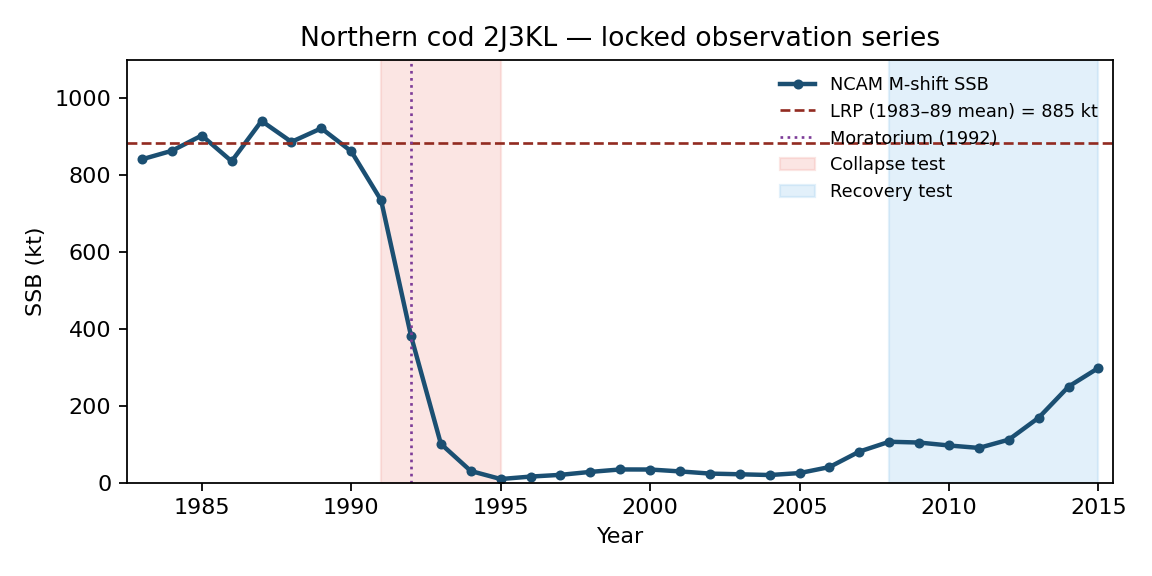
\includegraphics[width=\linewidth]{figs_e1/fig1_series.png}
\caption{NCAM M-shift SSB (DFO, 2016, Table A2). Dashed line: 2016 LRP = 884.6 kt. 2015 SSB is 33.8\% of that LRP, matching the advisory report statement of 34\%.}
\end{figure}

\begin{figure}[htbp]
\centering
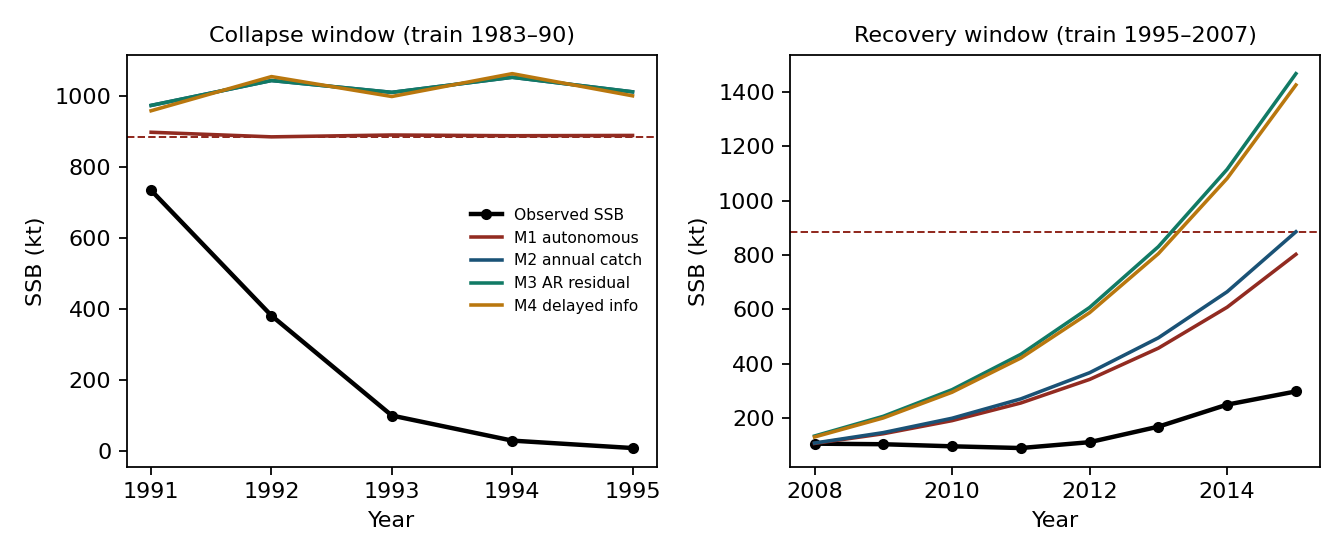
\includegraphics[width=\linewidth]{figs_e1/fig2_windows.png}
\caption{Multi-step forecasts from the end of each training window. Recovery is under-predicted when an AR residual fitted on a slow early-recovery train is persisted.}
\end{figure}

\textbf{Table 3.} Fixed-window scores (RMSE in kt), with both baselines
reported on every window, computed on the same fixed origins set
in Section 2.3. Table 3 is not to be read as a retention table ---
retention is decided on rolling-origin primary RMSE only.

\begin{longtable}[]{@{}llrrrrr@{}}
\toprule\noalign{}
Window & Model & RMSE & MAE & log-RMSE & Brier & Direction \\
\midrule\noalign{}
\endhead
\bottomrule\noalign{}
\endlastfoot
Collapse & persist & 670 & 610 & 2.71 & 0.00 & NA \\
& M1 & 694 & 638 & 2.73 & 1.00 & 0.50 \\
& M1b & 694 & 636 & 2.73 & 0.80 & 0.00 \\
& M2 & 819 & 751 & 2.85 & 1.00 & 0.25 \\
& M3 & 819 & 751 & 2.85 & 1.00 & 0.25 \\
& M4 & 819 & 750 & 2.85 & 1.00 & 0.25 \\
& mean & 688 & 630 & 2.72 & 0.00 & NA \\
Recovery & persist & 104 & 72 & 0.69 & 0.00 & NA \\
& M1 = M2 & 120 & 105 & 0.61 & 0.00 & 0.57 \\
& M1b & \textbf{90} & 55 & 0.52 & 0.00 & 0.57 \\
& M3 & 220 & 200 & 0.92 & 0.00 & 0.57 \\
& M4 & 214 & 195 & 0.91 & 0.00 & 0.57 \\
& mean & 144 & 124 & 1.60 & 0.00 & NA \\
\end{longtable}

On collapse, fitted \(r\) reaches \(1.935\), close to but not at the
imposed upper bound of \(2\).
The 1983--1990 window is a high, weakly trending stock. The fitted pre-collapse model does not reproduce the subsequent
decline, and dropping \(C\) from 240 to 5 raises forecast SSB. In the model the 1992 drop is supplied as an
exogenous catch path; historically it was largely a policy response to
depletion. Because production is stationary, prescribing the lower catch
in a constant-\(r\) stock-flow equation raises the predicted increment
and forces a mechanical rebound instead of reproducing the crash. Within this
accounting, had the crash been driven by the catch regime one would
expect supplying the catch path to help; M2 does not improve on M1. Supplying the prescribed catch path did not improve this
implementation's collapse-window hindcast. That is not proof of one
alternative: a misspecified and weakly identified module need not
improve even when the variable it adds is genuinely relevant, so the
result bounds what this ladder can attribute rather than identifying the
mechanism.

Under the coarse catch regime, M1 and M2 coincide on the recovery
window; under annual landings they do not (264 against 303 kt on the fixed recovery window, Section 3.2). The reason is structural:

On the recovery window (train 1995--2007, test 2008--2015) of
Specification A, M1 and M2 produce identical forecasts: M1 plugs the
training-mean catch into the autonomous map and M2 prescribes \(C_t\)
year by year, but \(C_t\equiv 5\) kt on both train and test windows, so
the two prescriptions coincide and the least-squares \((r,K)\) optimum is
identical.

M1b reports a lower RMSE (90 kt against M1's 120 kt), but
\(\mathfrak s\) descends towards zero and \(K\) settles just above the
training predictor range at \(105.8\) kt: an
unidentified Allee parameter, not a biological threshold. The estimate
approaches the lower boundary to numerical tolerance, for a reason visible in the objective.

\textbf{Observation 3.2 (Boundary Allee estimate on the recovery
window).} Any \(\mathfrak s\) strictly above the training minimum makes
the depensation factor
\(a(S_t)=(S_t-\mathfrak s)/(K-\mathfrak s)\) negative for observations
below \(\mathfrak s\), so wherever the observed \(\Delta S\) is positive
at such a state the fit incurs a large squared residual. On the
1995--2007 recovery window seven of the twelve annual increments are
positive --- the five negative ones fall in a single consecutive run,
1999--2004 --- and on balance this penalty pushes the estimate downward: the fitted \(\mathfrak s\)
descends towards zero (\(2.1\times10^{-23}\) under the coarse regime and
\(9.4\times10^{-6}\) under annual landings) while \(r\) reaches its
upper bound of \(2\) and \(K\) settles just above the training range at
\(105.8\) kt. Zero is excluded by the objective's feasibility
restriction \(0 < \mathfrak s < 0.8K\), so these values are a numerical
approach to an unattained infimum rather than an attained boundary
estimate. At such values the fitted object is effectively the
zero-threshold cubic branch \(a(S)=S/K\) of Definition 2.1, not a
positive-threshold Allee model, so M1b's lower error here is not
evidence for depensation: \(r\) and \(K\) absorb what \(\mathfrak s\)
does not.

This is an empirical finding about these fits, not a theorem, and we do
not state it as one. Two qualifications matter. The pressure just
described is a tendency and not a proof that the global optimum must lie
below the training minimum: the objective trades errors across all
observations, and \(r\), \(K\) and \(\mathfrak s\) can compensate (for M1b the catch is
plugged, not estimated, and the profile re-optimises only \(r\) and
\(K\))
for one another. The window is also not monotone --- SSB declines in
five consecutive annual decreases, from \(34.59\) kt in 1999 to
\(20.07\) kt in 2004, before rising to \(81.10\) kt in 2007 --- so no argument that
assumes a monotone recovery applies to it. Nor is a boundary estimate by
itself proof of non-identifiability, and a biologically meaningful
threshold may lie outside the sampled range.

A profile of the least-squares objective shows how weakly the data
constrain \(\mathfrak s\). The grid for \(\mathfrak s\) spans the profile range
\([0, \min_{\mathrm{train}} S_t] = [0, 9.68]\) kt. Two different ranges are in play and should not be conflated. Both are
built from the \emph{predictor} states of the training window --- the
\(S_t\) that the one-step regression conditions on, which exclude the
terminal response --- so on the recovery window (states 1995--2007) the
relevant maximum is \(S^{\mathrm{pred}}_{\max} = 40.83\) kt over the
twelve transitions beginning 1995--2006, not the \(81.10\) kt terminal
state of 2007.

\begin{longtable}[]{@{}lll@{}}
\toprule\noalign{}
Quantity & Range & Recovery window \\
\midrule\noalign{}
\endhead
\bottomrule\noalign{}
\endlastfoot
\(K\) & \([S^{\mathrm{pred}}_{\max}+10,\ 5000]\) kt & \([50.83,\ 5000]\) kt \\
\(\mathfrak s\), scored fit & \((0,\ S^{\mathrm{pred}}_{\max}]\), open at zero & \((0,\ 40.83]\) kt \\
\(\mathfrak s\), profile & \([0,\ \min_{\mathrm{train}} S_t]\) & \([0,\ 9.68]\) kt \\
\end{longtable}

The profile is computed on the narrower range so that the production
multiplier is non-negative at every predictor state. That is an
interpretive restriction adopted for the profile, not a feasibility
condition of the model and not a statistical ground for excluding higher
thresholds: a negative multiplier can be compatible with negative
observed increments, and the objective trades errors across
observations. Both ranges therefore exclude
a threshold placed above the collapsed range: at \(\mathfrak s = 50\) kt
--- outside the scored bound --- the factor \(a(S)\) would be negative
at all twelve predictor states, so the model would predict negative
production across the whole window. The estimate at the lower edge is
consequently a statement about a restricted feasible set, and this
design neither supports nor excludes depensation hypotheses --- a
predator pit, for instance --- that place the stock below a high
threshold throughout the recovery. Testing one requires lifting the
range bound, which is outside the frozen specification scored here. Fixing
\(\mathfrak s\) on that grid and re-optimising \(r\) and \(K\) at each
value gives a profile objective that rises only from \(126.50\) to
\(135.04\) kt\textsuperscript{2} under the coarse regime, and from
\(122.90\) to \(126.50\) kt\textsuperscript{2} under annual landings. Expressed as
\(n_{\mathrm{tr}}\log\{\mathrm{SSE}(\mathfrak s)/
\mathrm{SSE}(\hat{\mathfrak s})\}\) with \(n_{\mathrm{tr}}=12\), the
largest deviation across the grid is \(0.78\) under the coarse regime
and \(0.35\) under annual landings. We report these as descriptive
measures of curvature rather than as calibrated likelihood-ratio tests:
the least-squares fit carries no error model, the estimate
\(\hat{\mathfrak s}\) lies on the boundary of its range, \(r\) rests
at its own upper bound, the window supplies twelve transitions, and the
states are assessment reconstructions rather than direct observations.
Any one of these would compromise a \(\chi^2_1\) reference. The
substantive reading does not depend on the reference distribution: the
objective is nearly flat across the whole range, so the data do not
locate \(\mathfrak s\) within it.

The mechanism is parameter compensation. In
\(a(S_t)=(S_t-\mathfrak s)/(K-\mathfrak s)\), raising \(\mathfrak s\)
reduces the numerator while lowering \(K\) raises \(1/(K-\mathfrak s)\),
and along the profile \(K\) slides from \(106.0\) to \(82.7\) kt
(coarse) or \(129.8\) to \(95.6\) kt (annual landings) while \(r\)
remains at its upper bound of \(2\) throughout. The product
\(rS_t(1-S_t/K)\,a(S_t)\) is nearly invariant along this path, so the
data cannot separate \(\mathfrak s\) from \(K\). The training
observations therefore do not constrain behaviour near a putative
threshold, and the boundary estimate is not evidence about a biological
Allee threshold in either direction.

M3's \(\phi=0.95\) persists a negative residual, which raises its error
relative to persistence on this window; against its own declared
comparator M2 it still reads lower.

\begin{figure}[htbp]
\centering
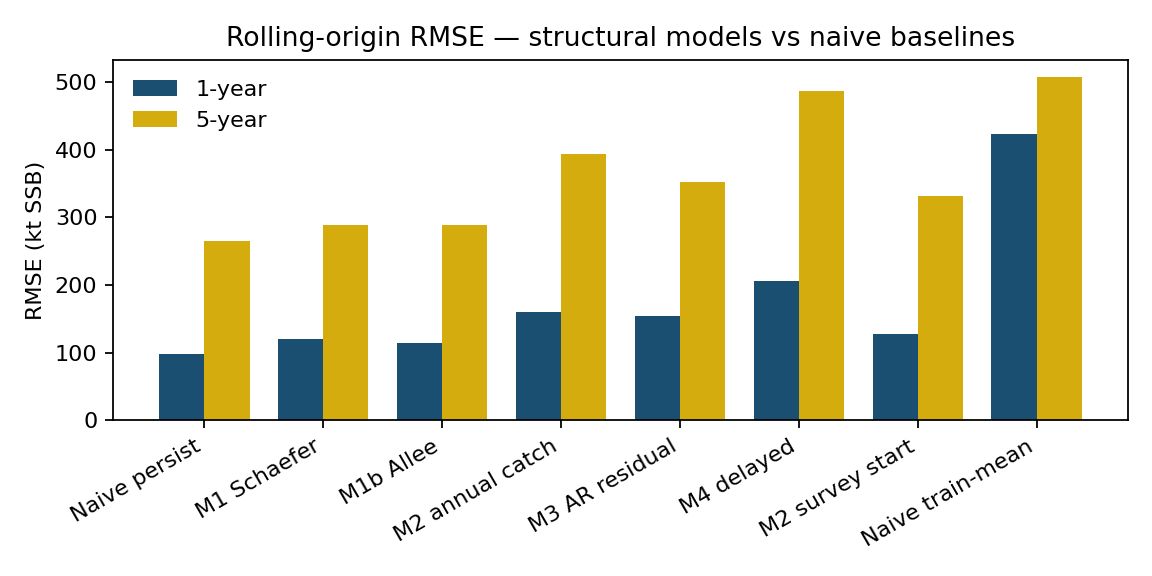
\includegraphics[width=\linewidth]{figs_e1/fig3_rmse.png}
\caption{Rolling-origin RMSE. Persistence is the best one-year and five-year point forecast.}
\end{figure}

\textbf{Table 4.} Rolling-origin summary, Specification A, coarse catch
regime.

\begin{longtable}[]{@{}lrrrr@{}}
\toprule\noalign{}
Model & \(h=1\) RMSE & \(h=1\) MAE & \(h=1\) log-RMSE & \(h=5\) RMSE \\
\midrule\noalign{}
\endhead
\bottomrule\noalign{}
\endlastfoot
persist & \textbf{98} & \textbf{48} & \textbf{0.52} & \textbf{265} \\
M1 & 121 & 80 & 8.02 & 289 \\
M1b & 115 & 80 & 8.70 & 289 \\
M2 & 144 & 61 & 0.59 & 398 \\
M3 & 135 & 53 & 3.39 & 366 \\
M4 & 196 & 82 & 0.76 & 488 \\
mean & 424 & 375 & 2.35 & 507 \\
\end{longtable}

Log-RMSE for M1 and M1b is large because some origins produce
trajectories that hit the numerical floor. M2 keeps the state off zero
and stabilizes the log score, but loses on raw RMSE. M4, the only model started from a year-old state, is the worst
structural model on raw RMSE; its decomposition against a stale-start
persistence control is reported in Section 4.

No structural model --- M1 through M4 --- is retained on Specification
A. Persistence is the lowest-RMSE forecast.

\subsubsection{3.2 Annual landings and survey
start}\label{annual-landings-and-survey-start}

Year-by-year landings for 2015 are 4.436 kt, matching DFO reported
landings. Pre-collapse catches are 172--269 kt, not a flat 240. The 1992
drop is to 41 kt, then 11 kt, then 0.4--1.9 kt.

\textbf{Table 5.} Rolling-origin RMSE (kt) with annual landings.

\begin{longtable}[]{@{}lrr@{}}
\toprule\noalign{}
Model & \(h=1\) & \(h=5\) \\
\midrule\noalign{}
\endhead
\bottomrule\noalign{}
\endlastfoot
persist & \textbf{98} & \textbf{265} \\
M1 & 121 & 289 \\
M1b & 115 & 289 \\
M2 & 160 & 394 \\
M3 & 154 & 352 \\
M4 & 206 & 486 \\
M2, survey start & 128 & 331 \\
\end{longtable}

Annual landings make M2 worse than the coarse regime on one-year RMSE
(160 versus 144 kt). Collapse-window RMSE under annual landings remains
about 821 kt for M2, M3 and M4 (819 kt under the coarse regime; M1 and
M1b are at 694 kt on both treatments, Table 3). On the annual-catch recovery window (train 1995--2007, test 2008--2015)
the ladder scores M1 264, M1b 78, M2 303, M3 609, and M4 586 kt, against
a frozen-persistence error of 104 kt (forecast held at the 2007 level of
81 kt). Annual landings therefore do not repair the recovery-window fit,
and the residual-persistence models deteriorate severely (609 and 586 kt
against 220 and 214 kt under the coarse regime). M1b's 78 kt carries the
same unidentified-Allee caveat as its regime-window fit.

Apparent net production \(S_{t+1}-S_t+C_t\) is strongly negative in
1991--93 even after subtracting reconstructed catch. This quantity is a
diagnostic construct, not an exact stock balance, and we do not treat it
as one: \(S\) here is spawning-stock biomass while \(C_t\) is total
landings, and changes in SSB also reflect maturation into the spawning
stock, changing maturity and weight-at-age schedules, and the age
composition of catch and of natural deaths. Within the surplus-production
accounting the ladder itself assumes --- in which \(S\) is the modelled
biomass state and \(C_t\) is subtracted from it --- matching the observed
\(\Delta S\) with no production at all would require removals of order
\(-\Delta S\), and the observed decline is far larger than \(C_t\). On
that reading the unexplained term dwarfs the difference between the two
catch treatments.
Regular et al.'s \(M \approx 2.5\) peak is an age-structured assessment's
estimate informed by additional data and assumptions; it is not the same
object as this scalar residual, though the two point in the same
direction. Within the model class tested, substituting annual recorded landings
for the coarse regime does not produce the crash in a constant-\(r\)
surplus model.

Reading the same quantity as an implied productivity makes the
non-stationarity explicit. Inverting the Schaefer form at a fixed \(K\)
gives \(\hat r_t = P_t / [S_t(1-S_t/K)]\), a reconstruction of
productivity rather than a forecast model. Periods below are labelled by the year in which a transition starts, so
the last usable transition begins in 2014. At \(K = 1032.7\) kt the
annual-landings series averages \(+1.82\) over the eight transitions
beginning 1983--1990, turns negative through 1991--1994 (mean
\(-0.79\), all four negative), and reads \(+0.37\) over 1995--2007
(thirteen) and \(+0.25\) over 2008--2014 (seven). At \(K = 5000\) kt the
sign pattern is the same --- \(+0.32\), \(-0.55\), \(+0.36\),
\(+0.22\) --- but the magnitudes are not: the post-collapse mean is
\(0.20\) of the pre-collapse mean at the fitted \(K\) and \(1.12\) of
it at \(K = 5000\) kt. The robust feature is therefore the sign
reversal, not the size of the pre-to-post contrast, and no constant
\(r\) reproduces a sequence that changes sign.
The ratio is undefined only at \(S_t = 0\) and \(S_t = K\); for
\(S_t > K\) it remains defined but its denominator is negative, so the
reading as a positive productivity fails. The coarse-regime recovery-window fit, whose
\(K\) is 500 kt, therefore cannot be read this way over the pre-collapse
states at all, since those states exceed its \(K\); the reconstruction
above uses the collapse-window \(K = 1032.7\) kt and the
annual-landings \(K = 5000\) kt, both of which exceed every observed
state.

\begin{figure}
\centering
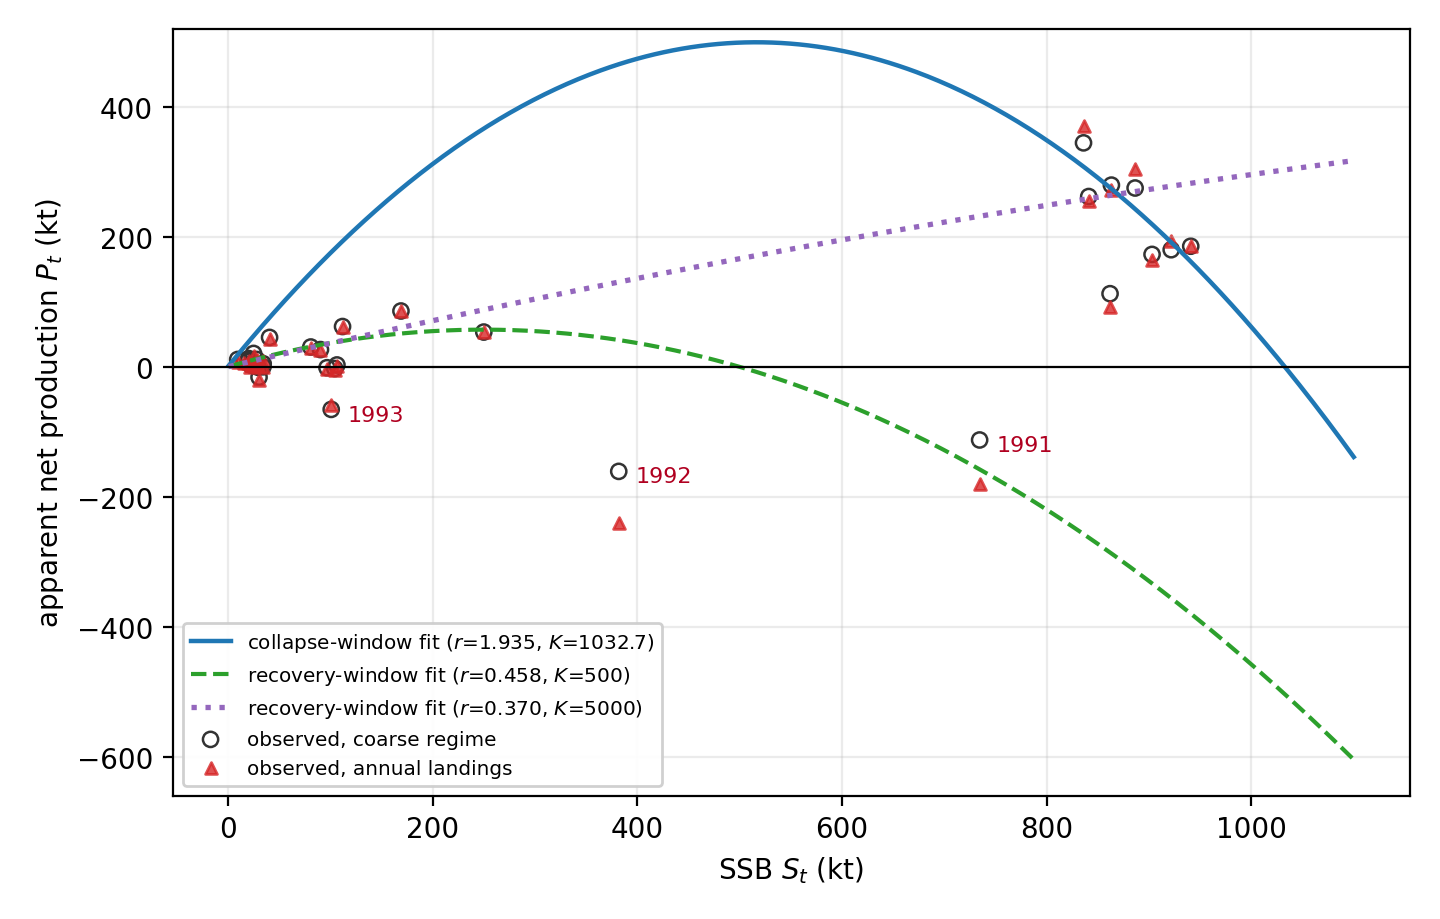
\includegraphics[width=\linewidth]{figs_e1/fig4_production.png}
\caption{Apparent net production \(P_t = S_{t+1}-S_t+C_t\) against \(S_t\)
under both catch treatments, with the fitted collapse-window and the two
recovery-window Schaefer curves overlaid. \(P_t\) is a diagnostic
construct, not a closed biomass budget: it inherits any error in the
catch reconstruction and any assessment revision in the SSB series, and
it is not a mass balance. The 1991--1993 points lie below every fitted
curve under both treatments, and the two recovery-window
parameterisations are almost indistinguishable over the observed range
of \(S_t\) while diverging widely when extrapolated beyond it.}
\label{fig:production}
\end{figure}

One numerical disclosure travels with the window: the annual-landings M1
(264 kt) and M1b (78 kt) differ from the coarse-regime recovery rows (M1
= 120, M1b = 90) although both treatments sit on the same SSB column.
The reconciliation is that M1's constant catch is not estimated on that
column. It is the training mean of the catch file: 5.0 kt for the coarse
regime, and 3.19 kt (the 1995--2007 mean of the annual landings) for the
annual treatment. The two least-squares objectives are nearly flat at
their minima (MSE 128.35 versus 127.84 kt\textsuperscript{2}), so the
\((r, K)\) minimizer slides along the valley as the constant changes:
\(r = 0.458\) with \(K\) resting at the multi-start initialiser of
500.0 kt --- not a bound, the lower bound on this window being 50.8 kt
--- against \(r = 0.370\) with \(K\) at its upper bound, 5000.0 kt. The optimiser leaves \(K\) at its starting value in this fit; the
profile of Section 3.2, not the optimiser's behaviour, is what
measures the flatness. The
same geometry explains the M1b pair (\(r\) pinned at its
upper bound in both treatments; \(K = 105.8\) against 129.8 kt): the
dependence of the M1b fit on the catch file is the flat-objective
identification of a two-parameter autonomous fit on a 13-year window,
not an inconsistency between fitting objects. The same flat valley caps what the ranking can resolve. Refitting the
recovery-window Schaefer map with \(K\) fixed anywhere on
\([60, 5000]\) kt and \(r\) re-optimised moves the one-step training
objective only from mean squared error \(127.4\) to \(149.9\) kt\(^2\)
(training RMSE \(11.29\)--\(12.24\) kt, a spread under \(0.95\) kt),
while \(r\) compensates from \(0.435\) to \(0.773\). On this window the
\((r, K)\) pair is not identified, and the ordering of valley variants
is not a robust ranking.

The collapse window is weakly identified in the complementary direction,
though less severely than the recovery window. There the stock is high
and weakly trending under large catch, so the data approximately impose
the single condition \(rS(1-S/K)\approx C\) on two parameters. Refitting
with the estimator of Section 2.3 at fixed \(K\) --- the same objective
on increments, the same bounds and multi-start --- raises the training
root mean squared error from \(31.3\) kt at the fitted
\(K = 1032.7\) kt to \(56.3\) kt at \(K = 1500\) kt and \(67.0\) kt at
\(K = 5000\) kt, while \(r\) falls from \(1.935\) to \(0.674\) and
\(0.331\). The objective therefore does discriminate here: a more than
twofold rise in training error is not a flat ridge. What the window does
not do is pin the pair tightly enough for the implied curve maxima to
agree, and the two windows fail in complementary directions --- a stock
near \(K\) constrains the product more than \(r\), and low-biomass
observations constrain \(K\) only weakly, because the density-dependent
term \(\partial g/\partial K = rS^{2}/K^{2}\) is small relative to the
approximately linear component rather than absent.

The implied maxima of the fitted curves make the consequence concrete.
The formal maximum \(rK/4\) and the reference state \(K/2\) of each
printed parameterisation are \(500\) kt and \(516\) kt for the collapse
window, \(57\) kt and \(250\) kt for the coarse-regime recovery fit, and
\(463\) kt and \(2500\) kt for the annual-landings recovery fit. These
are maxima of the fitted scalar curves, not sustainable-yield estimates
for this stock: the accounting caveat above --- SSB net of catch is not
a closed biomass budget --- applies to them unchanged. A spread of under
\(1\) kt in recovery-window training RMSE nevertheless separates curves
whose formal maxima differ by an order of magnitude. The fitted \(r\) is
correspondingly hard to read as a demographic rate: in this discrete
annual map the low-biomass multiplier is \(1+r\), so \(r = 1.935\)
corresponds to an annual factor of \(2.94\) and a continuous-equivalent
\(\log(1+r) = 1.08\,\mathrm{yr}^{-1}\), which is high for a
late-maturing gadoid but is not the same quantity as a continuous-time
intrinsic rate of increase, and SSB can also change through maturation
of existing cohorts. These are identification limits with biological
content, not numerical curiosities. One mechanism
unifies both faces of the catch-dependence: a constant catch shifts the
flat valley's minimiser without moving the objective, so the rolling
M1 and M1b scores (refit at every origin) are insensitive to the catch
treatment --- both are identical after the displayed rounding across the two
treatments (the archived values differ by at most 0.04 kt), because
future catch is not supplied to these modules --- though the
training-mean catch does change with treatment and can move their fitted
parameters, leaving the rolling scores at 121 and 115 kt at
\(h=1\) --- while the single
fixed-window fit is not. The property is specific to the two
constant-catch modules: M2, M3 and M4 take \(C_t\) into the state
update at every step, and their one-year rolling scores do move with the
treatment (144 to 160, 135 to 154, and 196 to 206 kt respectively).

Starting from \(\hat q I_t\) instead of SSB gives one-year RMSE 128 kt
(still worse than persist 98); one-year log-RMSE 0.49 versus persist
0.52; five-year RMSE 331 versus persist 265. On the primary score the
variant is not retained. The log-score difference is recorded and not
used for selection. The survey index contributes to NCAM and therefore
does not provide an independent validation target.

\subsubsection{3.3 Alternative assessment
specification}\label{alternative-assessment-specification}

\begin{figure}[htbp]
\centering
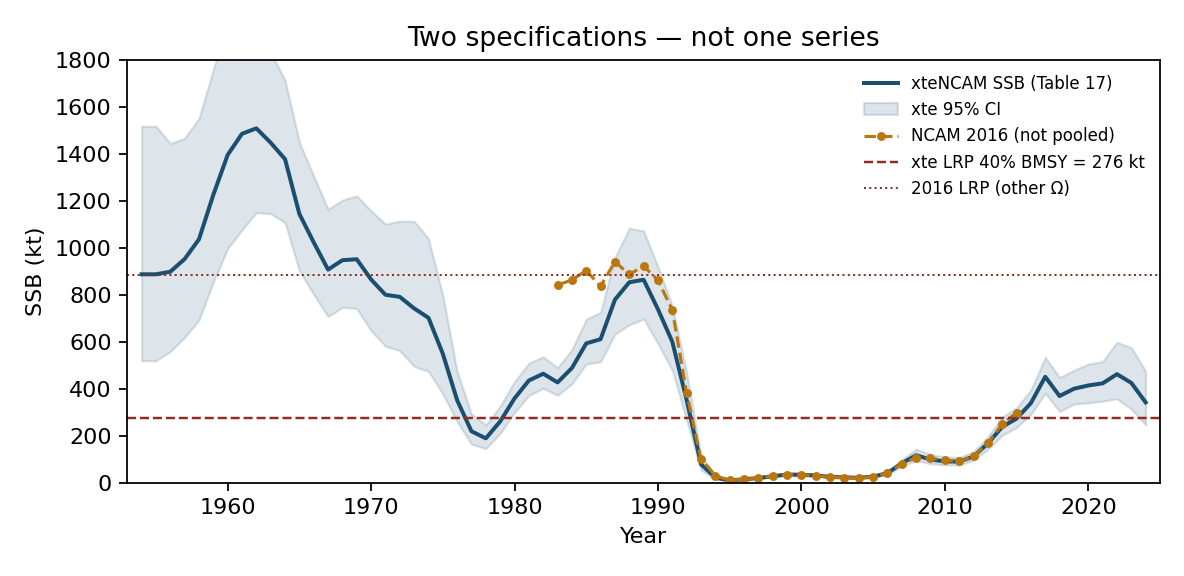
\includegraphics[width=\linewidth]{figs_e1/fig5_xtencam.png}
\caption{The two specifications. Overlap 1983--2015 RMSE = 126 kt (2015: NCAM 299 kt, xteNCAM 273 kt). Different safe sets. Not pooled.}
\end{figure}

Checkpoints from Regular et al.~(2025) Table 17: 2005 SSB = 26 kt (95\%
interval 22--31), 2017 = 451 kt (381--534), 2021 = 423 kt (NCAM and
xteNCAM said to agree), 2024 = 342 kt (246--475), 2024/LRP = 1.24. The
2005 values (26 kt versus NCAM 25.18 kt) can agree on a low year without
the two series sharing a reference point; agreement on a low year does
not warrant splicing the two columns. The 2015 value is
33.8\% of the old LRP, and the series is above the new one after 2016.

\textbf{Table 6.} Rolling-origin RMSE on Specification B (kt). The
persistence and training-mean rows are the origin-matched baselines,
computed on the ladder's own origin sets (\(n=59\) at \(h=1\),
\(n=55\) at \(h=5\)); the mixed-origin baselines over the longer naive
origin sets (\(n=63\) and \(n=59\)) are 88 and 318 kt for persistence
and 449 and 506 kt for the training mean.

\begin{longtable}[]{@{}lrr@{}}
\toprule\noalign{}
Model & \(h=1\) & \(h=5\) \\
\midrule\noalign{}
\endhead
\bottomrule\noalign{}
\endlastfoot
persist & \textbf{84} & \textbf{300} \\
M1 & 120 & 432 \\
M1b & 152 & 446 \\
M2 & 166 & 1059 \\
M3 & 127 & 930 \\
M4 & 206 & 1031 \\
mean & 458 & 522 \\
\end{longtable}

Collapse window (train 1954--89, test 1990--95): M1 RMSE 817 kt; M2 1898
kt. Official landings worsen the crash forecast. No module is retained.
Persistence remains the lowest-RMSE forecast. This is a second non-retention outcome under the same rule on a
different specification, and it is weaker than a statistical null
result. The longer series and the revised LRP
do not justify retaining the additional modules.

Recovery-stall window (train 1995--2012, test 2013--2024; \(n=12\)): M1
254 kt, M1b 178 kt, M2 269 kt, M3 268 kt, M4 269 kt. The 2013--2024 test
path rises from 167 kt to a 2022 peak of 462 kt before easing to 342 kt
in 2024, all above the 112 kt training-end value,
so a persistence forecast frozen at that value errs by 262 kt --- more
than M1 and M1b on this single origin. This fixed-origin comparison does
not enter the retention rule, which is decided on rolling-origin primary
RMSE (Table 6, where persistence is not beaten at either horizon). M1b's
window fit carries the identification fragility familiar from its other
window fits: a small fitted Allee parameter
(\(\mathfrak s = 5.3\times10^{-3}\)) with a carrying capacity (\(K=500\)
kt) extrapolated far beyond the training range (maximum 117 kt).

On the rolling Brier score for \(\mathbf{1}\{\hat S<\mathrm{LRP}\}\) on
Specification B (the secondary score, LRP = 276 kt):
persistence, on its origin-matched sets, \(4/59 = 0.07\) at \(h{=}1\)
and \(16/55 = 0.29\) at \(h{=}5\) (the same counts over the longer naive
origin sets give \(4/63 = 0.06\) and \(16/59 = 0.27\)); M1 0.05 and 0.45;
M1b 0.15 and 0.47; M2 0.07 and 0.36; M3 0.02 and 0.31; M4 0.07 and 0.38.
M1 and M3 improve the one-year Brier score over persistence (0.05 and
0.02 versus 0.07); no model improves it at \(h{=}5\), and no model
improves the primary RMSE score at either horizon (Table 6), so the
retention verdict is unchanged. For reference, the same secondary score on Specification A is 0.00 at
both horizons for persistence. The persistence indicator forecasts
\(\mathbf{1}\{S_t<884.6\}\) from the origin state, and its score is zero
because every origin state is already below the 884.6-kt LRP. In
particular the first origin, \(S_{1990}\), lies below the 1983--89 mean
bound, so the collapse train starts on the downslope of its own
reference period. The target years 1991--2015 are below the LRP as well,
so indicator and outcome agree at every origin. (The bare fact that targets are below the LRP
would not by itself make the persistence indicator correct; the origin
states being below it does.) Persistence supplies no directional prediction, so its sign-hit rate
is reported as NA rather than as a zero hit rate. The structural
scores are M1 0.04/0.05, M1b
0.00/0.05, M2 0.08/0.14, M3 0.08/0.10, M4 0.08/0.14 --- none below
persistence, which scores zero there by construction, and reported only to keep the two specifications' records
separate and complete.

Regular et al.~assign the 1992--94 disappearance primarily to \(M\)
(peak \(\approx 2.5\)), informed by tagging and a capelin/cod predictor,
and note that some of that \(M\) could still be unreported \(F\). The
relation between that attribution and the scalar residual of this ladder
is stated in Section 3.2.

\subsubsection{3.4 Prey-informed
productivity}\label{prey-informed-productivity}

Murphy et al.~(2025) report a 1991 acoustic collapse (1985--90 median
3704 kt versus 1991--2022 median 174 kt). A two-regime \(r\) with break
1991 uses the high regime only for forecasts issued before 1991. Capelin
enters as a candidate disturbance class, not as a fitted parameter.

\textbf{Table 7.} Rolling RMSE, two-regime \(r\). Baselines are origin-matched to the module's own origin sets (Specification A \(n=25/21\); Specification B \(n=59/55\)); the mixed-origin Specification B values over the longer naive sets are 88 and 318 kt.

\begin{longtable}[]{@{}llrr@{}}
\toprule\noalign{}
Specification & Model & \(h=1\) & \(h=5\) \\
\midrule\noalign{}
\endhead
\bottomrule\noalign{}
\endlastfoot
A & persist & \textbf{98} & \textbf{265} \\
A & M\_cap & 154 & 334 \\
B & persist & \textbf{84} & \textbf{300} \\
B & M\_cap & 147 & 894 \\
\end{longtable}

On post-break origins only (Specification B, \(h=1\); \(n=33\)): M\_cap
107 versus persistence 75 on the identical origin set (the all-origins value
of 88 is quoted in the Table 6 caption). Not retained. On Specification A post-break
origins (\(n=24\)) the corresponding M\_cap value is 149 kt.

The year-by-year 3L spring acoustic biomass is tabulated in the
Northwest Atlantic Fisheries Centre's Zenodo record (2025),
10.5281/zenodo.17515115, with 2023 = 331.3 kt from Murphy et al.~(2025).
Because \((I_{\mathrm{known}}/I_{\mathrm{ref}})^{b}>0\) for any
positive index value and any sign of \(b\), the scaled surplus keeps the
sign of \(g(S_t)\): the module can shrink production but cannot make it
negative, so food limitation severe enough to drive a net loss lies
outside what this specification can represent. Surplus is scaled by
\((I_{\mathrm{known}}/I_{\mathrm{ref}})^{b}\),
where \(I_{\mathrm{known}}(t)\) is the last observation at or before
\(t\), subject to the regime rule of Section 2. The index is carried forward from the last observation available at the
origin, and the carry is reset at 1991 only when the last observation
predates the break: an origin at or after 1991 with no post-1991
observation yet is not evaluated. Origins before 1991 draw on pre-break
surveys and are evaluated, so on Specification B the module is scored
from 1988 (\(n=36\) at \(h=1\), \(n=32\) at \(h=5\), of which three
origins precede the break); on Specification A the first eligible origin
is 1991 (\(n=24\) and \(n=20\)). Training transitions with no eligible
index value are dropped, and pre-1991 index observations are admissible
in training for pre-break origins on the same rule. Along a multi-step trajectory \(t\) is the forecast
year being stepped to, not the origin, so a five-year path may use index
values published after its issue date; this is a conditional hindcast
with respect to the index and is not an operational forecast. \(I_{\mathrm{ref}}\) is the training-window median of the
observed index, and \(b\) is a third free parameter fitted jointly with
\(r\) and \(K\) by one-step least squares on the training window. The
module additionally faces degrees-of-freedom starvation: three
parameters (\(r, K, b\)) are fitted on as few as eight training years at
the shortest origins, and after dropping years with no carried index
value the shortest fit uses only six one-step transitions (origin 1991
on Specification A, 1988 on Specification B; the estimator refuses to
fit on fewer) which invites in-sample overfitting and penalizes
the one-year out-of-sample comparison. Survey years are unobserved in
part of the record, so the index-forecast origins number \(n=24\)
(\(h=1\)) and \(n=20\) (\(h=5\)) on Specification A and \(n=36\) and
\(n=32\) on Specification B, against the SSB-based rolling-origin counts
(\(n=25\) at \(h=1\) and \(n=21\) at \(h=5\) on Specification A; Section
4).

\textbf{Table 8.} Rolling RMSE, observed acoustic index. Bold marks the
origin-matched baseline, which is the valid comparison for the module;
the mixed-origin rows over the longer naive origin sets are retained for
reference and are not the comparator. At \(h=5\) on Specification A
the module (262 kt) reads below the mixed-origin baseline (265 kt); that
apparent 3-kt advantage is an origin-mix artefact and is not marked,
because the origin-matched baseline on the module's own origins is
193 kt. The comparison that matters is the matched one.

\begin{longtable}[]{@{}llrr@{}}
\toprule\noalign{}
Specification & Model & \(h=1\) & \(h=5\) \\
\midrule\noalign{}
\endhead
\bottomrule\noalign{}
\endlastfoot
A & persist (mixed origins) & 98 & 265 \\
A & persist (origin-matched) & \textbf{97} & \textbf{193} \\
A & M\_cap\_index & 150 & 262 \\
B & persist (mixed origins) & 88 & 318 \\
B & persist (origin-matched) & \textbf{79} & \textbf{288} \\
B & M\_cap\_index & 132 & 492 \\
\end{longtable}

On the origin-matched reading the five-year near-tie on Specification A
dissolves --- the baseline on the module's own origins reads 193 kt
against the module's 262 kt --- and one-year RMSE is worse under both
readings (150 versus 98 kt on the SSB origins and 97 kt on the
module's); on Specification B the module's 132/492 kt stand against
origin-matched baselines of 79/288 kt. The module is not retained under
either baseline reading.

The scope of that result is set by the transmission the module encodes.
The index scales contemporaneous surplus, so what is tested is whether
prey information available at the origin improves the next steps through
a proportional change in aggregate production. Published maturity
schedules for this stock place the age at 50\% maturity between ages
five and six (Cadigan, 2016), so the pathway from a prey-driven change in
recruitment to a change in spawning-stock biomass is delayed by roughly
half a decade, and a contemporaneous multiplier cannot carry it. The same
timing objection applies to M4, whose one-year stale start is an
information delay rather than a recruitment delay. Non-retention here is
therefore evidence about the tested transmission and its timing, not
evidence that prey availability is unimportant to this stock.

\subsubsection{3.5 Uncertainty on the retention
margins}\label{uncertainty-on-the-retention-margins}

The uncertainty analysis attaches descriptive Diebold--Mariano loss-differential statistics
(Diebold and Mariano, 1995; unweighted HAC truncation at lag \(h-1\)) and
moving-block bootstrap intervals (K\"unsch, 1989; block length
\(\max(h,3)\), 20,000 replications, seeded) to the retention margins of
the retention rule. It is computed from the archived per-origin forecast
files: on Specification B the xteNCAM rolling file; on Specification A
the layer is computed on the primary coarse-regime pass. Its per-origin
rows were regenerated from the registered estimator and archived; the
regeneration reproduces the archived annual-landings per-origin file
and the archived coarse-regime summary exactly, so no score changes.
Recomputing the layer on the annual-landings pass, which earlier
editions used, leaves every interval reading unchanged.
The persistence baseline is not archived per-origin; it is recomputed on the
identical origin sets from the registered series, and the recomputation
reproduces the recorded origin-matched baselines (98 and 265 kt on
Specification A; 84 and 300 kt on the matched Specification B origins)
--- the script fails loudly otherwise. The moving-block intervals quantify sampling variation in the archived
origin-level loss sequence conditional on the fitted forecast paths; they
are not predictive intervals and do not propagate parameter-estimation,
assessment-revision, catch-reconstruction or covariate uncertainty. The
layer attaches uncertainty to margins the point rule has already
ranked; it changes no frozen verdict,
score, or table value.

The two columns of Table 9 summarise the same comparison through
different approximations. The DM statistic \(z\) tests the mean of the
per-origin squared-loss differential \(d_i = L_{A,i} - L_{B,i}\) against
zero, scaled by a HAC standard error. The interval and \(p\) come from
the moving-block bootstrap of the difference of RMSEs,
\(\sqrt{\overline{L_A}} - \sqrt{\overline{L_B}}\). The two effect
measures are monotonically related, since
\(\sqrt{\overline{L_A}}-\sqrt{\overline{L_B}} =
(\overline{L_A}-\overline{L_B})/(\sqrt{\overline{L_A}}+
\sqrt{\overline{L_B}})\), so they share a sign and a zero null; the
square root rescales the gap but does not by itself make one summary
more stable than the other. What differs is the approximation used to
gauge sampling variability --- a HAC-scaled asymptotic normal reference
against a resampling distribution over blocks --- and in samples this
small and this dependent the two need not agree. Four of the
twenty-eight rows have an interval excluding zero while \(|z| < 1.96\)
(Specification A \(h=1\) M4 against M3; Specification B \(h=1\) M3
against persistence; Specification B \(h=5\) M1b against persistence and
M4 against M3; see Section SI-3). We therefore report the two
summaries side by side
and do not treat the bootstrap interval as a second calibrated test. The interval and the \(p\) are mutually
consistent in every row. The quantity reported as \(p\) is the percentile-tail fraction
\(2\min\{\#(\Delta^{*}_b\le 0),\ \#(\Delta^{*}_b\ge 0)\}/B\) over the
\(B\) block-resampled differences, obtained by inverting the percentile
interval rather than from a null-centred resampling scheme; it is an
interval-based summary and not a calibrated test of a sharp null, and a
reported value of zero means no resampled difference fell on the
opposite side of zero; where the two columns disagree we
report both and rest no verdict on either.

Because the origins overlap at \(h=5\), the estimation window expands,
the predictand is a smoothed reconstruction and the sample straddles a
structural break, the automatic \(h-1\) HAC truncation and the
\(\max(h,3)\) block length should not be taken as neutral choices. The
M1-against-persistence margin was therefore recomputed over a grid of
both (Section SI-3). The DM statistic crosses the conventional
threshold within the range of defensible bandwidths, upward on
Specification A and downward on Specification B, so nothing rests on it;
the bootstrap is markedly more stable across block lengths \(3\) to
\(9\). The qualitative reading --- Specification A within noise,
Specification B separating --- is therefore a bootstrap result rather
than a DM result, established for that comparison and not asserted for
every module. Read
``within noise'' as ``this analysis does not resolve the difference'',
not as evidence that the models are equivalent.

\textbf{Table 9.} Uncertainty on the retention margins. Both
specifications are scored on their primary pass: Specification A rows
are the coarse catch regime, so the RMSE values reproduce Table 4, and
Specification B rows are the xteNCAM rolling pass.
(Diebold--Mariano with HAC lag \(h-1\); K\"unsch moving-block
bootstrap, block length \(\max(h,3)\), 20,000 replications, seeded).
Gaps are module minus comparator, in kt; positive gaps mean the module
is worse.

\begin{longtable}[]{@{}
  >{\raggedright\arraybackslash}p{(\columnwidth - 20\tabcolsep) * \real{0.0750}}
  >{\raggedleft\arraybackslash}p{(\columnwidth - 20\tabcolsep) * \real{0.1000}}
  >{\raggedright\arraybackslash}p{(\columnwidth - 20\tabcolsep) * \real{0.0750}}
  >{\raggedright\arraybackslash}p{(\columnwidth - 20\tabcolsep) * \real{0.0750}}
  >{\raggedleft\arraybackslash}p{(\columnwidth - 20\tabcolsep) * \real{0.1000}}
  >{\raggedleft\arraybackslash}p{(\columnwidth - 20\tabcolsep) * \real{0.1000}}
  >{\raggedleft\arraybackslash}p{(\columnwidth - 20\tabcolsep) * \real{0.1000}}
  >{\raggedleft\arraybackslash}p{(\columnwidth - 20\tabcolsep) * \real{0.1000}}
  >{\raggedleft\arraybackslash}p{(\columnwidth - 20\tabcolsep) * \real{0.1000}}
  >{\raggedright\arraybackslash}p{(\columnwidth - 20\tabcolsep) * \real{0.0750}}
  >{\raggedleft\arraybackslash}p{(\columnwidth - 20\tabcolsep) * \real{0.1000}}@{}}
\toprule\noalign{}
\begin{minipage}[b]{\linewidth}\raggedright
Spec
\end{minipage} & \begin{minipage}[b]{\linewidth}\raggedleft
\(h\)
\end{minipage} & \begin{minipage}[b]{\linewidth}\raggedright
Module
\end{minipage} & \begin{minipage}[b]{\linewidth}\raggedright
Comparator
\end{minipage} & \begin{minipage}[b]{\linewidth}\raggedleft
\(n\)
\end{minipage} & \begin{minipage}[b]{\linewidth}\raggedleft
RMSE module
\end{minipage} & \begin{minipage}[b]{\linewidth}\raggedleft
RMSE comp.
\end{minipage} & \begin{minipage}[b]{\linewidth}\raggedleft
Gap (kt)
\end{minipage} & \begin{minipage}[b]{\linewidth}\raggedleft
DM \(z\)
\end{minipage} & \begin{minipage}[b]{\linewidth}\raggedright
95\% CI (kt)
\end{minipage} & \begin{minipage}[b]{\linewidth}\raggedleft
\(p\)
\end{minipage} \\
\midrule\noalign{}
\endhead
\bottomrule\noalign{}
\endlastfoot
A & 1 & M1 & persist & 25 & 120.5 & 98.0 & +22.5 & 1.13 & {[}\ensuremath{-}13.4, +52.2{]} & 0.192 \\
A & 1 & M1b & persist & 25 & 114.8 & 98.0 & +16.8 & 0.98 & {[}\ensuremath{-}19.4, +59.6{]} & 0.384 \\
A & 1 & M2 & persist & 25 & 144.1 & 98.0 & +46.0 & 1.29 & {[}\ensuremath{-}12.3, +83.0{]} & 0.452 \\
A & 1 & M3 & persist & 25 & 134.6 & 98.0 & +36.6 & 0.99 & {[}\ensuremath{-}16.8, +64.2{]} & 0.932 \\
A & 1 & M4 & persist & 25 & 195.6 & 98.0 & +97.5 & 1.53 & {[}\ensuremath{-}9.1, +172.7{]} & 0.278 \\
A & 1 & M2 & M1 & 25 & 144.1 & 120.5 & +23.5 & 0.91 & {[}\ensuremath{-}60.7, +66.9{]} & 0.684 \\
A & 1 & M4 & M3 & 25 & 195.6 & 134.6 & +60.9 & 1.21 & {[}+4.4, +134.4{]} & 0.000 \\
A & 5 & M1 & persist & 21 & 288.7 & 264.7 & +24.0 & 1.84 & {[}\ensuremath{-}43.1, +56.4{]} & 0.279 \\
A & 5 & M1b & persist & 21 & 288.6 & 264.7 & +23.9 & 1.84 & {[}\ensuremath{-}43.1, +56.4{]} & 0.284 \\
A & 5 & M2 & persist & 21 & 398.2 & 264.7 & +133.5 & 1.10 & {[}\ensuremath{-}21.0, +217.5{]} & 0.421 \\
A & 5 & M3 & persist & 21 & 366.4 & 264.7 & +101.6 & 1.12 & {[}\ensuremath{-}0.8, +151.4{]} & 0.078 \\
A & 5 & M4 & persist & 21 & 488.2 & 264.7 & +223.5 & 1.14 & {[}\ensuremath{-}20.8, +409.4{]} & 0.405 \\
A & 5 & M2 & M1 & 21 & 398.2 & 288.7 & +109.5 & 0.98 & {[}\ensuremath{-}77.1, +232.8{]} & 0.805 \\
A & 5 & M4 & M3 & 21 & 488.2 & 366.4 & +121.9 & 1.15 & {[}\ensuremath{-}27.4, +263.2{]} & 0.707 \\
B & 1 & M1 & persist & 59 & 119.5 & 84.4 & +35.0 & 2.81 & {[}+2.7,
+70.8{]} & 0.032 \\
B & 1 & M1b & persist & 59 & 151.6 & 84.4 & +67.2 & 3.60 & {[}+18.3,
+117.7{]} & 0.009 \\
B & 1 & M2 & persist & 59 & 166.0 & 84.4 & +81.6 & 3.22 & {[}+36.4,
+122.8{]} & 0.000 \\
B & 1 & M3 & persist & 59 & 126.7 & 84.4 & +42.3 & 1.85 & {[}+1.0,
+92.5{]} & 0.042 \\
B & 1 & M4 & persist & 59 & 205.7 & 84.4 & +121.3 & 3.20 & {[}+53.7,
+193.0{]} & 0.000 \\
B & 1 & M2 & M1 & 59 & 166.0 & 119.5 & +46.6 & 1.78 & {[}\ensuremath{-}20.5,
+104.5{]} & 0.170 \\
B & 1 & M4 & M3 & 59 & 205.7 & 126.7 & +79.0 & 3.07 & {[}+35.6,
+116.4{]} & 0.000 \\
B & 5 & M1 & persist & 55 & 431.9 & 300.0 & +131.9 & 2.06 & {[}+33.2,
+218.6{]} & 0.008 \\
B & 5 & M1b & persist & 55 & 445.5 & 300.0 & +145.5 & 1.80 & {[}+18.2,
+250.9{]} & 0.023 \\
B & 5 & M2 & persist & 55 & 1058.9 & 300.0 & +758.9 & 2.15 & {[}+363.6,
+1038.5{]} & 0.000 \\
B & 5 & M3 & persist & 55 & 930.1 & 300.0 & +630.2 & 2.39 & {[}+352.8,
+845.6{]} & 0.000 \\
B & 5 & M4 & persist & 55 & 1030.7 & 300.0 & +730.8 & 2.35 & {[}+407.3,
+978.3{]} & 0.000 \\
B & 5 & M2 & M1 & 55 & 1058.9 & 431.9 & +627.0 & 1.97 & {[}+195.7,
+929.7{]} & 0.004 \\
B & 5 & M4 & M3 & 55 & 1030.7 & 930.1 & +100.6 & 1.88 & {[}+20.2,
+177.4{]} & 0.007 \\
\end{longtable}

Splitting the same origins by period rather than by horizon shows what
the pooled score aggregates. On Specification B at \(h=1\), computed on
the archived per-origin records with no refit, persistence reads
\(94.7\) kt before 1991 (\(n=26\)) against \(142.4\) kt for M1;
\(167.0\) kt across 1991--1995 (\(n=5\)) against \(126.8\) kt for M1
and \(66.6\) kt for M1b; \(20.7\) kt across 1996--2012 (\(n=17\))
against \(19.7\) kt for M3; and \(61.0\) kt from 2013 (\(n=11\))
against \(96.4\) kt for M3. These rolling scores answer a different question from the fixed-window
collapse test of Section 3.1, where models fitted on 1983--1990 are
asked whether a pre-collapse fit anticipates the crash, and none does.
Here each forecast is issued from an origin already inside the decline,
with training extended to that origin, so the question is whether the
next year is closer to a refitted model or to the last observed state; a
one-step forecast issued in 1993 from an already-collapsed state is not
evidence that a model predicted the collapse. On that second question
persistence is the lowest-error forecast in the two quiescent bands but
not in the collapse band, where the structural modules read below it on
five origins; leave-one-out on
that band leaves M1 below persistence in all five cases, so the ordering
is stable, though five origins remain too few to score. The
1996--2012 margin is \(0.93\) kt on a \(20.67\)-kt baseline, inside the
\(5\%\) tie band of \(1.03\) kt and with a bootstrap interval of
\([-14.2, +14.9]\) kt that includes zero: a tie under the stated rule,
not a win. No retention verdict changes, because the rule scores pooled
rolling RMSE at both horizons and the one sub-band advantage falls
inside the band the rule declares non-deciding. The reading that changes
is interpretive: the pooled result combines regimes in which persistence
wins by a wide margin with a collapse band in which it does not, so the
non-retention statement is a statement about the pooled score rather
than about every period of this series.

Readings. On Specification A no non-retention margin against persistence separates
from zero. At \(h=1\) the deficits against persistence (16.8--97.5 kt
on \(n=25\)) carry DM \(z\) from 0.98 to 1.53 with bootstrap \(p\) from
0.19 to 0.93; at \(h=5\) (23.9--223.5 kt on \(n=21\)) \(z\) runs from
1.10 to 1.84 with \(p\) from 0.08 to 0.42. The heavy-tailed
collapse-window losses dominate the bootstrap variance at this sample
size, so the Specification A outcome is a point-rule ranking whose
margins lie within noise: the scores suffice to order the models and do
not resolve small skill differences. On Specification B the non-retention
separates: every module's deficit against persistence has a bootstrap interval excluding zero at
\(h=1\) (\(p\) from 0.042 to below 0.001 on \(n=59\)) and at \(h=5\)
(\(p\) at most 0.023 on \(n=55\)). The declared (H1) comparators behave
asymmetrically: M2's deficit against M1 is within noise at \(h=1\) on
both specifications and at \(h=5\) on Specification A, with the interval excluding zero only
on Specification B at \(h=5\) (\(p=0.004\)), while M4's delay cost
against M3 separates at \(h=1\) on both specifications (\(p\) below
0.001) and at \(h=5\) on Specification B (\(p=0.007\)) but not on
Specification A (\(p=0.71\)). The alternative comparator rows are held in the archive rather than
printed in Table 9. On the primary passes they read: Specification A
\(h=1\), gap \(+29.3\) kt, \(z=0.91\), interval
\([-67.6, +82.8]\) kt; \(h=5\), \(+109.7\) kt, \(z=0.98\),
\([-77.1, +232.8]\) kt; Specification B \(h=1\), \(+14.4\) kt,
\(z=0.51\), \([-67.5, +89.1]\) kt; \(h=5\), \(+613.4\) kt,
\(z=1.93\), \([+170.9, +945.1]\) kt. Accordingly, on them the reading (M2
against M1b) is within noise at \(h=1\) on both specifications and at
\(h=5\) on Specification A, separating on Specification B at \(h=5\)
(\(p=0.005\)): the comparator declaration of the retention rule is
immaterial to every recorded verdict, as the protocol disclosure
records. The layer is produced by a registered script, deterministic under seed 0,
with its output archived alongside it; Section SI-3 names both.

\subsubsection{3.6 Fitted parameters}\label{fitted-parameters}

This section collects in one place every fitted-parameter value the
article prints, the window or treatment it belongs to, and the bound it
attains. The table collects values reported in the preceding
sections; nothing is recomputed. Quantities not reported individually
(the per-origin rolling fits of every module, the index module's
per-window exponent \(b\), and the delay module's structural setting)
are held in the archive rather than
invented. The collection exists so the identification record --- bounds
attained, interior fits, the flat valley --- can be read at a glance.

\textbf{Table 10.} Fitted parameters, with the section in which each is
reported.

\begin{longtable}[]{@{}
  >{\raggedright\arraybackslash}p{(\columnwidth - 6\tabcolsep) * \real{0.2500}}
  >{\raggedright\arraybackslash}p{(\columnwidth - 6\tabcolsep) * \real{0.2500}}
  >{\raggedright\arraybackslash}p{(\columnwidth - 6\tabcolsep) * \real{0.2500}}
  >{\raggedright\arraybackslash}p{(\columnwidth - 6\tabcolsep) * \real{0.2500}}@{}}
\toprule\noalign{}
\begin{minipage}[b]{\linewidth}\raggedright
Module
\end{minipage} & \begin{minipage}[b]{\linewidth}\raggedright
Window / treatment
\end{minipage} & \begin{minipage}[b]{\linewidth}\raggedright
Fitted values
\end{minipage} & \begin{minipage}[b]{\linewidth}\raggedright
Bound / identification status
\end{minipage} \\
\midrule\noalign{}
\endhead
\bottomrule\noalign{}
\endlastfoot
M1 & Collapse, Specification A (train 1983--1990) (\S{}3.1, \S{}4) &
\(r = 1.935\), \(K = 1032.7\) kt, constant catch \(240\) kt; repeller
\(144\) kt, attractor \(889\) kt, monotone below \(783\) kt,
\(F'(S^*) \approx -0.39\) & \S{}3.1 records the collapse-window fitted
\(r\) as constrained near, but not attaining, the upper bound of \(2\) \\
M1 & Recovery, coarse catch regime (\S{}3.2) & \(r = 0.458\), constant
catch \(5.0\) kt (the training mean); training MSE \(128.35\) kt\textsuperscript{2}
& \(K\) at \(500.0\) kt, the multi-start initialiser, not a bound (the
lower bound on this window is \(\max_{\mathrm{train}}S + 10 =
50.8\) kt) \\
M1 & Recovery, annual landings (\S{}3.2) & \(r = 0.370\), constant catch
\(3.19\) kt (the 1995--2007 landings mean); training MSE \(127.84\)
kt\textsuperscript{2} & \(K\) at its upper bound, \(5000.0\) kt \\
M1b & Recovery, coarse catch regime (\S{}2.2, \S{}3.2) &
\(\mathfrak{s} = 2.1\times10^{-23}\), \(r = 2.000\),
\(K = 105.8\) kt & \(\mathfrak{s}\) approaches lower bound to numerical tolerance; \(r\)
pinned at its upper bound in both treatments; \(K\) a valid interior
fit \\
M1b & Recovery, annual landings (\S{}3.2) &
\(\mathfrak{s} = 9.4\times10^{-6}\), \(r = 2.000\),
\(K = 129.8\) kt & \(\mathfrak{s}\) at the lower boundary to
numerical tolerance \\
M1b & Recovery-stall, Specification B (train 1995--2012) (\S{}3.3) &
\(\mathfrak{s} = 5.3\times10^{-3}\), \(K = 500\) kt, training-window
maximum \(117\) kt & identification fragility: \(\mathfrak{s}\)
small, \(K\) extrapolated far beyond the training range \\
M3 & Rolling, Specification A (\S{}3.1) & \(\phi = 0.95\) (AR(1) residual
coefficient) & printed value; the per-window rolling \(\phi\) values are
archive items \\
\texttt{M\_cap\_index} & Index module (\S{}3.4) & \(r\), \(K\), \(b\) fitted jointly by
one-step least squares & fitted values not printed (archive);
degrees-of-freedom note at \(n = 8\) training years \\
M1 & Flat-valley sweep, recovery window (\S{}3.2) & \(K\) fixed
anywhere on \([60, 5000]\) kt moves the one-step training objective only
from MSE \(127.4\) to \(149.9\) kt\textsuperscript{2} (training RMSE \(11.29\)--\(12.24\)
kt) while \(r\) compensates over \([0.435, 0.773]\) & the \((r, K)\)
pair is not identified on this window; the ordering of valley variants
is not a robust ranking \\
M4 & Rolling, all specifications & \(r\), \(K\), \(\phi\) refitted by
the same procedure as M3 at every origin; the module adds no parameter
of its own, the one-year delay being structural & archive: the refitted
per-origin values coincide with M3's and are not printed separately \\
All modules & Per-origin rolling fits & archive items (not printed);
M1b's Specification B rolling Allee optimum is environment-sensitive at
the \ensuremath{\pm}17 kt level (\S{}Data availability) & --- \\
\end{longtable}

Bounds: \(r \in (0.001, 2]\), and \(K\) optimised on
\([\max_{\mathrm{train}} S + 10, 5000]\) kt, where the maximum is taken
over the states the one-step regression conditions on. On the
1995--2007 recovery window those are the years 1995--2006, with maximum
\(40.8\) kt, giving a lower bound of \(50.8\) kt. Optimisation starts
from \(K = 500\) kt. The recovery-window M1 fit reports \(K = 500.0\)
kt: the optimiser does not move from its starting value, which lies
\(449\) kt above the bound, because the objective is flat there. This is
the same flat-valley geometry quantified in Section 3.2, and a
stationary starting value is a sharper symptom of it than an active
bound would be.

\subsubsection{3.7 Operating characteristics of the retention
rule}\label{operating-characteristics}

The result above is negative, so its interpretation turns on whether the
rule could have detected added structure had it been present. That
question cannot be answered from the cod series alone. It was addressed
by a simulation study whose design --- data-generating processes,
replicate count, and the thresholds separating an adequate from an
inadequate rule --- was registered and archived before any synthetic
series was generated.

Five processes were simulated, each a member of the ladder's own class
and parameterised from the fitted values of Section 3.6, using the
estimation and trajectory code of Section 2.3 unmodified: an autonomous
Schaefer map at the collapse-window fit (D1) and at the recovery-window
fit (D2), a stock-flow map with the coarse regime path (D3), a
depensatory map with an identifiable threshold \(\mathfrak s = 15\) kt
(D4), and a persistence-true null with no surplus term (D5). Each was
run at \(\sigma = 11.8\) and \(33.8\) kt, the archived recovery- and
collapse-window residual standard deviations, on 33-year series matching
Specification A, with 200 seeded replicates per cell. The full retention
rule was applied unchanged.

\begin{longtable}[]{@{}llrr@{}}
\toprule\noalign{}
Process & Generating module & \(\sigma=11.8\) & \(\sigma=33.8\) \\
\midrule\noalign{}
\endhead
\bottomrule\noalign{}
\endlastfoot
D1 autonomous, collapse fit & M1 & 0.965 & 0.985 \\
D2 autonomous, recovery fit & M1 & 0.710 & 0.130 \\
D3 stock-flow & M2 & 0.090 & 0.110 \\
D4 depensation, \(\mathfrak s=15\) kt & M1b & 0.005 & 0.015 \\
D5 persistence-true & none retained & 0.985 & 0.970 \\
\end{longtable}

The first four rows give the proportion of replicates in which the
generating module was retained; the last gives the proportion in which
no structural module was retained when persistence was true. The
false-retention rate across all structural processes was \(0.044\).

Two properties follow. The rule is \emph{specific}: under a
persistence-true process it declines to retain structure in \(97\)--\(99\%\)
of replicates, so the empirical non-retention is not an artefact of an
instrument that rejects everything. It is also \emph{conditionally
powerful}: where the generating signal is strong, as in the
high-biomass, large-catch conditions of D1, it recovers the true module
in \(97\)--\(99\%\) of replicates.

Power is nevertheless low for three of the four structural processes.
In absolute terms the binding constraint is not the comparator gates:
requiring a module to beat persistence alone, ignoring H1 and the tie
band, already retains the true module in only \(33\%\) of D3 replicates
and \(18\%\) of D4 replicates, so the gates account for an absolute
\(0.17\)--\(0.23\) of the shortfall. Conditional on clearing that bar,
however, the comparator requirement is a dominant further filter,
removing \(69\%\) of surviving D3 replicates and \(94\%\) of surviving
D4 replicates; demanding that a module beat both persistence and its
declared comparator is substantially more stringent than demanding it
beat persistence alone.

The identification limit is clearer still in the raw scores. With five
structural modules, chance alone would make the generating module the
lowest-error one \(20\%\) of the time. It holds that position in
\(62.7\%\) of D1 and \(64.5\%\) of D2 replicates, but in only \(25.8\%\)
of D4 replicates and \(3.8\%\) of D3 replicates --- for the stock-flow
process, less often than if the winner were drawn at random, with a mean
one-year error (85.7 kt) above that of the residual (77.9 kt) and Allee
(79.9 kt) modules. On 33 annual observations at these parameters the
correct structure is not merely hard to detect; estimation noise
actively disadvantages it relative to its siblings.

The consequence for the empirical result is that its strength is not
uniform across modules. Had the collapse window been generated by an
autonomous map at the fitted parameters, the rule would have retained
M1 in \(97\%\) of replicates; it does not retain M1 on the observed
series, so those data are inconsistent with that generating process and
the non-retention is evidence about the stock rather than about the
instrument. Non-retention of the stock-flow and depensation modules
under recovery-window conditions is by contrast weak evidence against
those structures, because the rule would have retained them in at most
\(11\%\) and \(1.5\%\) of replicates even had they been true. The
residual and lagged-initialisation modules were not simulated as
generating processes, so no power estimate is available for them; their
power is plausibly bounded by the stock-flow figure, since both extend
the same base map and must clear an additional comparator, but that is
an inference rather than a measurement.

Two limits are inherent to the design and were recorded with it. The
processes are members of the ladder's own class, so this measures power
against correctly specified alternatives and the D1 figure is an upper
bound; and the synthetic predictand carries no assessment smoothing, so
persistence is a weaker baseline here than on the reconstructed series.

The same rule has been applied to a groundwater system, the Edwards
Aquifer, in Abaee (2026a), and the comparison isolates a property that
this series cannot show. There the autonomous module reads below
persistence on the point ranking at one year (12.84 against 13.23 ft)
and is still not retained, because the margin falls inside the 5\% tie
band and reverses at five years (21.25 against 21.11 ft). On the present
series no module comes within the band at either horizon: the closest
approach is M1b at \(9.0\%\) adrift at five years and \(17.1\%\) at one
year, against a band of \(5\%\). The two cases therefore reach the same verdict by
different routes: here the ranking alone decides, whereas on the
groundwater series the tie band and the two-horizon requirement are what
withhold retention from a module the point rule would have kept. Neither
series is pooled with the other and no verdict is transferred; what
recurs is the decision rule, not the data or the outcome.

That companion also records a distinction worth stating here. A module
may improve the score and still not constitute added structure: the
groundwater stock-flow variant fitted with training-mean fluxes beats
persistence at one year yet was declined on the ground that it collapses
to an autoregression when those fluxes are held constant. M1b raises the
same question in a different form. Its fitted threshold descends towards
an unattained infimum, at which point the production term is the
zero-threshold cubic branch of Definition 2.1 rather than a
positive-threshold Allee model, so its lower error on Specification A is
not evidence for depensation. The scored rule does not encode this
distinction --- it compares errors --- and both cases are resolved by
inspecting what the fitted module has become, not by the score.

\subsection{4. Discussion}\label{discussion}

The observed path falls far below the fitted lower equilibrium and then
recovers. No exact fixed autonomous noise-free scalar trajectory can
reproduce that. The obstruction is structural, and is stated below for
the map held at constant catch; the scored collapse failure has a
simpler and more direct cause, given after the proposition.

\textbf{Proposition 4.1 (No recovery from below the lower equilibrium,
for autonomous noise-free scalar surplus maps).} \emph{Let
\(S_{t+1}=F(S_t)\) be an autonomous one-dimensional surplus-production
map of Definition 2.1 evaluated with \(\varepsilon_t \equiv 0\) and a
constant catch \(C_t \equiv C\), with at most two positive equilibria --- a lower
repelling point \(S_-\) and an upper attracting point --- and a one-step
map monotone below its maximum; the single-equilibrium monotone regime
is the special case, and the fitted collapse-window map (\(r = 1.935\),
\(K = 1032.7\) kt, constant catch \(240\) kt) has exactly this form
(repeller \(144\) kt, attractor \(889\) kt, monotone below \(783\) kt).
If the observed path \((S_t)\) falls strictly below \(S_-\) at some
time and is strictly larger at some later time, then no trajectory of
\(F\) reproduces \((S_t)\) exactly. The Specification A collapse path
satisfies the hypothesis: NCAM SSB falls to \(9.7\) kt by 1995, far
below the fitted repeller of \(144\) kt, and rises thereafter. }

The argument is immediate: below the lower equilibrium \(F(S) < S\), and
\([0, S_-)\) is forward-invariant because \(F\) is monotone there and
\(F(S_-) = S_-\), the interval being closed at the left because the
implementation clips the state at a non-negative floor. Every trajectory
entering \([0, S_-)\) therefore decreases toward the floor and never
returns above \(S_-\), so a path that goes below \(S_-\) and is later
higher is not a trajectory of \(F\).

Two limits on the scope of this proposition should be stated
explicitly, because both are easy to overstate. First, it does not say
that autonomous maps cannot produce non-monotone paths: the fitted map
has \(F'(S^\star) \approx -0.39\) at its attractor, so approach to the
attractor is by damped oscillation, and declines followed by recoveries
are the generic local behaviour there (from \(950\) kt the fitted map
gives \(950 \to 857 \to 899\) kt). What is excluded is recovery after a
fall below the lower repeller, which is the feature the observed
collapse path actually has. Second, the result is a statement about
autonomous noise-free scalar maps only. It does not apply to the
stochastic map of Definition 2.1 with \(\varepsilon_t \neq 0\), nor to
M3 and M4, which carry a residual state and a stale initial state
respectively and are therefore not autonomous scalar maps. The
proposition applies directly to M1 under the deterministic forecast
convention used here, and to M1b whenever its own fitted map has the
stated equilibrium structure. It does not formally cover M2, whose
prescribed year-by-year catch makes the update a time-indexed family
\(F_t\) rather than a single autonomous map; for M2 the argument is
motivating rather than binding, and the collapse-window result of
Section 3.1 is the relevant evidence. It is not an impossibility
theorem for surplus-production modelling in general.

A third limit is the most consequential for ecological reading, and it
follows from the same algebra. The lower equilibrium is generated by the
removals, not by any depensatory term in the production function. For
the Schaefer map the positive equilibria of \(rS(1-S/K)=C\) are
\(S_{\pm}(C) = (K/2)\left[1 \pm \sqrt{1-4C/(rK)}\right]\), so the
repeller is a function of catch: at the fitted \(r = 1.935\),
\(K = 1032.7\) kt it sits at \(144\) kt under \(C = 240\) kt, at
\(66\) kt under \(C = 120\) kt, and at \(2.6\) kt under the
moratorium-level \(C = 5\) kt, approaching zero as \(C\) does. The
1995 SSB of \(9.7\) kt is far below the first of these and above the
last. The obstruction is therefore a statement about a stock held under
sustained removals of the pre-collapse magnitude; it is not evidence of
biological depensation, and it does not explain non-recovery after
catches fell. Nothing in Definition 2.1's Schaefer branch contains an
Allee effect --- that is the separate M1b branch --- so a threshold
recovered from an M1 fit should not be read as a biological one.

The collapse forecasts fail for a more direct reason than the
equilibrium structure. Every module carries stationary production, so
each predicts positive surplus at the biomass levels of the late 1980s
while the reconstruction falls. For the modules supplied with the catch
path --- M2, M3 and M4 --- the 1992 decline in prescribed catch raises
the predicted increment directly, so they turn upward exactly where the
reconstruction turns down; M1 and M1b use a training-mean constant and
turn upward because that constant is smaller than the losses the
reconstruction records. That mechanism, not the crossing of a
catch-dependent repeller computed at \(C = 240\) kt, is what the
fixed-origin collapse scores record.

The fixed-window sign-hit rates of \(\Delta S\) for the structural
modules (0.00--0.50 on collapse; NA for the baselines, which supply no
directional prediction; Table 3) record the directional character of that failure: the
structural models miss not only the magnitude of the crash but the sign
of the trajectory exactly when the official catch series drops.

Under both the coarse catch regime and official landings, lowering \(C\)
in 1992 cannot generate the crash. Neither prescribed catch treatment reproduced the reconstructed decline
in these implementations; which process accounts for the shortfall ---
productivity, unallocated mortality, or the observation and
reconstruction of the series --- is not identified by this comparison.
Nor does this test whether fishing caused the historical collapse: in
this accounting \(S_t\) is spawning-stock biomass while \(C_t\) is total
landings, which is not an age-structured removal from the spawning
stock, so the exercise bounds a scalar catch-driven surplus story and
not the causal role of the fishery. That is
compatible with DFO's caution that NCAM \(M\) can absorb unreported
deaths: the crash remains such an event under the best available public
catch reconstruction, which tightens that limitation rather than
relaxing it.

Unidentified extra structure does not close the gap to persistence, and
in two of the five structural modules (M2 and M4) it widens it. The direction is not uniform
and should not be stated as though it were: relative to its own declared
comparator M3 reads below M2 in all six rolling comparisons (by 6 to 129
kt), and M1b reads below M1 at \(h=1\) on Specification A and on the
fixed recovery window, though not on Specification B, where M1b is the
higher of the two (152 against 120 kt at \(h=1\)). What fails is H2, not always H1. Where the added
structure does hurt, the mechanism is visible: autoregressive residuals
fitted on short, regime-changing windows persist the wrong sign, an
Allee parameter goes to the boundary, and a one-year delay removes
information. These modules stay descriptive unless the conditions under
which a module's contribution could be certified rather than merely
scored hold.

The 2016 LRP is the 1980s mean SSB, so over its own reference years the
mean deviation of SSB from that bound is zero by construction, though
individual annual deviations are not. Defining the threshold from the
same years that a leading-indicator claim would be tested on does not
establish prospective early-warning performance for 1983--1990.

The moratorium is a change in implementable catch and is already in
\(C_t\). A separate delay switch does not add a degree of freedom beyond
stock-flow. Whether the 1992 management architecture admits any feasible
catch path that keeps the stock above its reference threshold is a
separate question from one-year forecast error, treated for this stock
in Abaee (2026c), and is not addressed
here.

One-dimensional surplus production is not NCAM: age structure,
migration, and survey catchability are omitted. The test is whether this
ladder is retained under the stated score, not whether the assessment is
a good filter. M4 is a stale-start experiment rather than a fully delayed information
set: its trajectory begins at \(S_{t-1}\), but its parameters are
M3's, fitted on training transitions that end at \(S_t\), so the
later state still reaches the forecast through the fitted coefficients
and the carried residual. Because the path starts one year earlier,
reaching a target \(h\) years after the origin takes \(h+1\) updates
rather than \(h\). The catch path is indexed from the earlier start, so
the first update applies \(C_{t-1}\), and the residual recursion is
applied before the first step, so the first projected residual is
\(\hat\phi\,e_{\mathrm{last}}\) where \(e_{\mathrm{last}}\) is the
residual of the transition \(S_{t-1}\to S_t\); the first update
therefore re-forecasts the transition on which that residual was fitted.
It is therefore a perturbed
initialisation evaluated at calendar time \(t\), not propagation from a
genuinely year-old information set. A genuinely delayed variant would truncate
training as well, and is not scored here. Its one-year gap against
persistence therefore mixes a stale initial state with the model's own
cost.

The separating control --- persistence issued from the last available
assessment, \(S_{t-1}\) --- decomposes the gap. On Specification A under
the coarse catch regime (the primary pass) the control reads 184.4 kt at
\(h = 1\) and 329.8 kt at \(h = 5\), against M4's 195.6 kt and 488.3 kt.
The information delay, the year-old start under the same persistence
rule, therefore accounts for 86.4 of the 97.5-kt one-year gap and the
surplus model's own cost for the remaining 11.1 kt; at \(h = 5\) the
split is 65.1 against 158.4 kt.

On Specification B every term is computed on M4's own origin set, so
that the control, the baseline and the module share origins (\(n=59\)
at \(h=1\), \(n=55\) at \(h=5\)). Matched persistence reads 84.4 and
300.0 kt and the stale-start control 158.0 and 337.4 kt, against M4's
205.7 and 1030.7 kt. The delay accounts for 73.6 of the 121.3-kt
one-year gap and the model's own cost for the remaining 47.7 kt; at
\(h = 5\) the model's own cost dominates (693.3 of 730.8 kt). These are descriptive comparisons between two
forecast rules, not a causal decomposition of the value of assessment
timeliness: the delayed control still reads off the same smoothed
reconstruction, and access to a later reconstruction is not the same
thing as access to a timely real-world assessment. With that reading,
M4's error is numerically dominated by the initialisation component at the
one-year horizon on both specifications, and mostly the surplus model's own structure at the
five-year horizon on Specification B: at \(h = 1\) the surplus model's
own penalty is only about 11 kt --- relative to the stale-start control the gap decomposes numerically into
an initialisation component and a residual-surplus component, an
arithmetic split between forecast rules rather than a causal
attribution. For reference, the one-year lag in the start state accounts for \(86.4\) kt
at \(h = 1\) on Specification A, against structural costs over timely
persistence of \(23\) kt for M1, \(17\) for M1b, \(46\) for M2 and
\(37\) for M3, and M4's own structure-given-delay cost of \(11.1\) kt.
These are differences between forecast rules on a smoothed
reconstruction and are not an estimate of the operational value of
assessment timeliness.

The predictand is an assessment smoother (NCAM/xteNCAM SSB), not a raw
observation: forecasting it is forecasting a filtered state, and
persistence inherits the smoother's autocorrelation --- the comparison
is valid for ``does this ladder track this assessment,'' not for a
vintage or early-warning reading, which would require assessment
vintages at each origin, and none is available. Persistence is
correspondingly not an empty null on this predictand. Spawning-stock
biomass aggregates surviving mature cohorts of a long-lived species, and
the assessment adds further temporal smoothing, so strong one-year
autocorrelation is the expected baseline on biological and observational
grounds alike. Beating it requires useful prediction of subsequent change, whether a
sustained trend or a transition such as the collapse, the onset of
rebuilding, or the post-2015 stall. Persistence is retained as the scoring benchmark the retention rule is
defined against, not as a biological projection, and no demographic
balance is asserted on its behalf at either horizon.
Recreational catch remains incompletely measured.

The log-RMSE scores of Table 4 carry a floor caveat: structural
trajectories absorb at the numerical floor
\(\varepsilon_{\mathrm{log}} = 10^{-3}\) kt rather than at zero (the
trajectory code clips the state to
\([\varepsilon_{\mathrm{log}}, 10^{6}]\) kt), and the reported values
use \(\log\max(\hat S, \varepsilon_{\mathrm{log}})\);
\(\varepsilon_{\mathrm{log}}\) is part of the registered scoring
configuration and is distinct from the process noise \(\varepsilon_t\)
of Definition 2.1. The floor binds often --- for M1 and M1b it binds on a majority of
five-year origins on both specifications --- and the per-origin counts
are given in Section SI-4. The raw-RMSE column is the retention score, so no retention verdict
depends on the floor; it affects the log column only, which is reported
as a secondary diagnostic. Recomputing that column with the floor
lowered to \(10^{-6}\) and \(10^{-9}\) leaves the log-RMSE ordering of
the five modules unchanged at both horizons on both specifications, so
no secondary ranking depends on it either. A constant-productivity map is
misspecified for a series whose assessment attributes the crash to
\(M \approx 2.5\); the test is whether that misspecification still
forecasts SSB better than persistence, and the scored comparison answers
that for this ladder on these series. Sample sizes are small
(\(n=33\) years on Specification A; rolling \(n=25\) at \(h=1\) and
\(n=21\) at \(h=5\)). They suffice to rank models and do not suffice to
certify a small skill difference. The 2023 40\% \(B_{\mathrm{MSY}}\) LRP
is the Specification B setting, and Section 3.3 is that review: the
ladder was run on the xteNCAM series under a fresh
specification-matching review, with the same non-retention verdict.

\textbf{Reconstruction-level corroboration.} An independent,
assessment-level record sharpens the same boundary. Rose (2026) compares
two surplus-production reconstructions of the stock spanning 1983--2023
--- the Rose and Walters (2019) model and the DFO (2024a) assessment
model --- and documents that surplus production and stock growth stalled
after 2015, with some years negative, the stall-point biomass being
controversial between the two reconstructions and well below historical
norms. The recovery-stall window of Specification B (train 1995--2012,
test 2013--2024) overlaps that period (its 2016--2024 portion). A stock
whose surplus production and stock growth stall together, with some
years negative and the stall-point biomass below historical norms ---
the configuration Rose (2026) reports --- is precisely the configuration
a constant-productivity surplus law cannot reproduce, and the ladder's
single-origin comparison on that window is consistent with it on the
rolling score, which is what decides retention. On that single fixed
origin M1 (254 kt) and especially M1b (178 kt) do read below frozen
persistence (262 kt); the retention verdict is nonetheless negative,
because it is decided on rolling-origin RMSE, where persistence is not
beaten at either horizon. The fixed-window result is reported because
selecting favourable episodes would tell a different story from rolling
evaluation, and that contrast is itself part of the finding. The two reconstructions' disagreement
at the stall point is moreover the assessment-level twin of the ladder's
own non-uniqueness: M1b's apparent recovery-window skill is carried by a
carrying capacity extrapolated far beyond the training range, exactly
the extrapolation on which the two reconstructions diverge. Rose (2026)
also documents the limit-reference-point trajectory --- successive
downward revisions to just over 0.3 Mt, then to about 0.25 Mt in 2025
--- which is the norm-field drift that separates the two specifications
evaluated here (884.6 kt versus 276 kt) and the reason their columns are
never pooled.

\textbf{Attribution and the prey modules.} Rose (2026) infers from
structural-equation models that the post-2015 production deficit is
limited by capelin and amplified by harp seal predation, with fishing
almost certainly not the sole cause. That attribution is consistent with
the ladder's two negative findings, and it sharpens both. First, it
matches the catch-treatment null: neither prescribed catch treatment
repairs the collapse, which is what one would expect if the dominant
missing term is not catch. Both treatments could omit relevant
removals, and other structural errors could prevent either from helping,
so the scored result is consistent with that attribution rather than
establishing it. Second, it draws the
identification boundary inside the prey results: capelin limitation can
be a real production driver --- the 1991 acoustic collapse is large
(1985--90 median 3704 kt versus 1991--2022 median 174 kt) --- while the
corresponding forecast modules still fail the stated score. A driver's
reality at the reconstruction level does not make it a usable forecast
module at the surplus-production level: the two-regime and
acoustic-index variants are weakly constrained by their short training
windows and missing index years, and they fail the retention score. No
parameter profile was computed for them, so their non-retention rests
on prediction error rather than on a demonstrated identification
failure.

\textbf{Protocol status.} The evaluation windows and the scoring core
--- the primary RMSE comparison and the persistence bar --- were coded
before the first scoring pass and applied unchanged. Two components of
the retention rule were not: the 5\% tie band and the comparator
declarations for the non-nested rungs were formalised after the scores
of Section 3 had been computed. Neither affects any outcome reported
here; the tie band never decides a retention result, the smallest deficit
being \(17.1\%\). The design is therefore a fixed computational
protocol, not a prospective registration, and the additional passes
(annual landings, survey start, capelin, Specification B) were declared
in the text as they were added. No dated pre-scoring protocol file exists for this study.
Section~SI-1 records the order in which each pass was run.

The results are specific to the objects tested. They do not extend to
other estimators of the same model family, to closed-loop filtering
schemes, or across the two assessment specifications, which are scored
separately throughout. The delay evaluated here is a one-year
information delay in the forecast start state, not a continuous-time
retarded system.

On this evidence, within the scope of this estimator and ladder, modules
that are not identified on the training data did not reduce forecast
error below matched persistence at both horizons here. Weak
identification is documented for the recovery-window Allee fits and is
not established as the sole cause of non-retention. The retained
forecast is persistence.

\subsection{5. Conclusions}\label{conclusions}

On locked NCAM M-shift SSB for 1983--2015, last-value persistence is
more accurate than surplus production, catch-driven stock-flow,
autoregressive residuals, delayed information, and prey-informed
productivity. The crash is not a catch-drop event in this accounting.
Extra structure did not recover the gap to persistence at both
horizons, and the stale-start module enlarged it; the autoregressive
module improved on its own declared comparator without closing the gap
to persistence. The same
retention outcome holds on the unpooled xteNCAM series, whose post-2015
stall period fails in the same way the reconstructions stall.

The paper reports a forecast comparison. It does not conclude that the
stock is unsustainable, and it does not conclude that the evaluation
framework is empirically confirmed on this stock.

\subsection{References}\label{references}

Abaee, A., 2026a. Does a one-pool water-balance model improve forecasts
of Edwards Aquifer head? A scored test at J-17. Zenodo.
https://doi.org/10.5281/zenodo.22552680.

Abaee, A., 2026b. Periodic review as sampled governance: sample-and-hold
dynamics of assessment-driven effort control, a selected 42-stock
spectral screen, and the Northern Cod case. Zenodo.
https://doi.org/10.5281/zenodo.22554297.

Abaee, A., 2026c. Robust viability of the 2J3KL limit reference point
under a surplus-production map: policy scoring, expansion, and when
catch cannot help. Zenodo. https://doi.org/10.5281/zenodo.22552060.

Cadigan, N.G., 2016. A state-space stock assessment model for northern
cod, including under-reported catches and variable natural mortality
rates. Can. J. Fish. Aquat. Sci. 73, 296--308.

Diebold, F.X., Mariano, R.S., 1995. Comparing predictive accuracy. J.
Bus. Econ. Stat. 13, 253--263.
https://doi.org/10.1080/07350015.1995.10524599

Carvalho, F., Winker, H., Courtney, D., Kapur, M., Kell, L., Cardinale,
M., Schirripa, M., Kitakado, T., Yemane, D., Piner, K.R., Maunder, M.N.,
Taylor, I., Wetzel, C.R., Doering, K., Johnson, K.F., Methot, R.D.,
2021. A cookbook for using model diagnostics in integrated stock
assessments. Fish. Res. 240, 105959.

DFO, 2009. A fishery decision-making framework incorporating the
Precautionary Approach. Fisheries and Oceans Canada, Ottawa.

DFO, 2016. Stock Assessment of Northern cod (NAFO Divs. 2J3KL) in 2016.
DFO Can. Sci. Advis. Sec. Sci. Advis. Rep.~2016/026.

DFO, 2024a. NAFO Divisions 2J3KL Northern Cod stock assessment to 2024.
DFO Can. Sci. Advis. Sec. Sci. Advis. Rep.~2024/049.

DFO, 2024b. Assessment of capelin in NAFO Divisions 2J3KL. DFO Can. Sci.
Advis. Sec. Sci. Advis. Rep.~2024/050.

Hutchings, J.A., Myers, R.A., 1994. What can be learned from the
collapse of a renewable resource? Atlantic cod, Gadus morhua, of
Newfoundland and Labrador. Can. J. Fish. Aquat. Sci. 51, 2126--2146.

Hyndman, R.J., Koehler, A.B., 2006. Another look at measures of forecast
accuracy. Int. J. Forecast. 22, 679--688.

Kell, L.T., Kimoto, A., Kitakado, T., 2016. Evaluation of the prediction
skill of stock assessment using hindcasting. Fish. Res. 183, 119--127.

Kell, L.T., Sharma, R., Kitakado, T., Winker, H., Mosqueira, I.,
Cardinale, M., Fu, D., 2021. Validation of stock assessment methods: is
it me or my model talking? ICES J. Mar. Sci. 78, 2244--2255.

Kokkalis, A., Berg, C.W., Kapur, M.S., Winker, H., Jacobsen, N.S.,
Taylor, M.H., Ichinokawa, M., Miyagawa, M., Medeiros-Leal, W., Nielsen,
J.R., Mildenberger, T.K., 2024. Good practices for surplus production
models. Fish. Res. 275, 107010.

K\"unsch, H.R., 1989. The jackknife and the bootstrap for general
stationary observations. Ann. Stat. 17, 1217--1241.
https://doi.org/10.1214/aos/1176347265

Murphy, H.M., Adamack, A.T., Lewis, R.S., Bourne, C.M., 2025. Assessment
of capelin in NAFO Divisions 2J+3KL to 2023. DFO Can. Sci. Advis. Sec.
Res. Doc. 2025/022.

Northwest Atlantic Fisheries Centre, 2025. 2J3KL cod and capelin biomass
indices. Zenodo. https://doi.org/10.5281/zenodo.17515115

Regular, P.M., et al., 2025. Assessment of the Northern Cod stock in
NAFO Divisions 2J3KL in 2024. DFO Can. Sci. Advis. Sec. Res. Doc.
2025/048.

Rose, G.A., 2026. Northern cod comeback: 10 years after. Can. J. Fish.
Aquat. Sci. 83, 1--14. https://doi.org/10.1139/cjfas-2025-0141

Rose, G.A., Rowe, S., 2015. Northern cod comeback. Can. J. Fish. Aquat.
Sci. 72, 1789--1798.

Rose, G.A., Walters, C.J., 2019. The state of Canada's iconic Northern
cod: a second opinion. Fish. Res. 219, 105314.

Schijns, R., Froese, R., Hutchings, J.A., Pauly, D., 2021. Five
centuries of cod catches in Eastern Canada. ICES J. Mar.~Sci. 78,
2675--2683.

Shelton, P.A., Healey, B.P., 1999. Should depensation be dismissed as a
possible explanation for the lack of recovery of the northern cod (Gadus
morhua) stock? Can. J. Fish. Aquat. Sci. 56, 1521--1524.

Walters, C., Maguire, J.-J., 1996. Lessons for stock assessment from the
northern cod collapse. Rev.~Fish Biol. Fish. 6, 125--137.

\section*{Declarations}

\subsection*{Data availability}

All input data, analysis scripts, result files, and the frozen model
specification are archived at
\url{https://github.com/MIKEAA2020/general-sustainability} and
\url{https://zenodo.org/records/22553609}.

\subsection*{Reproducibility}

All computations are deterministic: within a fixed interpreter and
library stack, repeated executions reproduce every result file byte for
byte. An independent re-execution verified all 29 recorded output
checksums and regenerated all 30 result files byte-identically; one
registered file carries no pinned checksum and is covered by the
regeneration comparison. Across environments, the intervention runners
and the OLS-based prediction runners regenerate their outputs byte for
byte, while the four optimizer-based forecast runners (L-BFGS-B fits)
reproduce every scored row at printed precision with one exception: the
M1b rolling row on Specification B, whose Allee optimum is
environment-sensitive at the \ensuremath{\pm}17 kt level (\(h=1\): 151.6
versus 153.2 kt; \(h=5\): 445.5 versus 462.5 kt, on Python
3.12/numpy 2.1.3/scipy 1.14.1 against the recorded original
environment). That sensitivity is consistent with the identification
fragility reported for M1b in Section 3.1 (\(\mathfrak s\) descending
towards zero, \(K\) resting at the 500-kt multi-start initialiser), and
it is immaterial to the retention verdict, which persistence wins at
both horizons by margins far larger than the instability. The archive
records the checksums of the original-environment outputs; the
deterministic-in-environment claim and this sensitivity note together
are the reproducibility statement.

The uncertainty layer of Section 3.5 is produced by a seeded,
deterministic script applying Diebold--Mariano (HAC) statistics and a
K\"unsch moving-block bootstrap to the archived per-origin forecast
files; the persistence baseline is recomputed there on the identical
origin sets from the registered series and asserted against the recorded
origin-matched values. The script and its output are archived with the
repository.

\begin{verbatim}
python3 src/run_ladder.py && python3 src/run_xte.py
python3 src/run_capelin_regime.py && python3 src/run_capelin_index.py
python3 src/compare_catch.py && python3 src/make_figures.py
\end{verbatim}

\subsection*{CRediT authorship contribution statement}

{[}To be completed at submission.{]}

\subsection*{Funding}

{[}To be completed at submission.{]}

\subsection*{Declaration of competing interest}

The authors declare that they have no known competing financial
interests or personal relationships that could have appeared to
influence the work reported in this paper.

\subsection*{AI declaration}
GLM (Z.ai), Qwen (Alibaba Cloud) and DeepSeek AI assisted with drafting and iterative review.

\end{document}
